
\documentclass[10pt,twocolumn,letterpaper]{article}

\usepackage{xeCJK}
\setCJKmainfont{SimSun}
\setCJKsansfont{SimHei}
\setCJKmonofont{FangSong}



\usepackage[pagenumbers]{cvpr}

\definecolor{cvprblue}{rgb}{0.21,0.49,0.74}
\usepackage{multirow}
\usepackage{arydshln}
\usepackage[pagebackref,breaklinks,colorlinks,allcolors=cvprblue]{hyperref}

\definecolor{Lavender}{RGB}{230, 230, 250}
\definecolor{indigo}{rgb}{0.294, 0.0, 0.51}

\def\paperID{7721}
\def\confName{CVPR}
\def\confYear{2025}

\newcommand{\fref}[1]{Figure~\ref{#1}}
\newcommand{\eref}[1]{(\ref{#1})}
\newcommand{\sref}[1]{Section~\ref{#1}}
\newcommand{\tref}[1]{Table~\ref{#1}}
\newcommand{\aref}[1]{Appendix~\ref{#1}}

\title{AirRoom: 物体在房间重识别中的重要性}

\author{
Runmao Yao \quad
Yi Du \quad
Zhuoqun Chen \quad
Haoze Zheng \quad
Chen Wang \\
Spatial AI \& Robotics (SAIR) Lab, University at Buffalo \\
{\tt\small \{yaorunmao, zhz19231211\}@gmail.com, \{yid, chenw\}@sairlab.org, zhc057@ucsd.edu}
}
\begin{document}
\maketitle
\begin{abstract}
房间重识别(ReID)是一项具有挑战性但至关重要的任务,广泛应用于增强现实(AR)和家庭护理机器人等领域。现有的视觉位置识别(VPR)方法通常依赖于全局描述符或聚合局部特征,但在拥挤的室内环境中,尤其是那些充满人造物体的环境中,常常难以有效工作。这些方法往往忽视了物体相关信息的关键作用。为了解决这一问题,我们提出了AirRoom,这是一种物体感知管道,整合了多层次的物体相关信息——从全局上下文到物体补丁、物体分割和关键点——并采用粗到细的检索方法。在四个新构建的数据集(MPReID、HMReID、GibsonReID和ReplicaReID)上的大量实验表明,AirRoom在几乎所有评估指标上都超越了最先进的(SOTA)模型,提升幅度从6\%到80\%不等。此外,AirRoom展现出显著的灵活性,允许管道中的各种模块被不同的替代方案替换,而不会影响整体性能。它还在不同视角变化下表现出强大且稳定的性能。项目网站:\href{https://sairlab.org/airroom/}{\textcolor[rgb]{0.3,0.5,1}{https://sairlab.org/airroom/}}。

\end{abstract}

\vspace{-5pt}
\section{Introduction}
\label{sec:intro}
\vspace{-2pt}

With the rapid development of spatial computing, room reidentification (ReID) has become a key area of interest, enabling advancements in applications like augmented reality (AR) \cite{schult2023controlroom3droomgenerationusing} and homecare robotics \cite{sarch2022tideetidyingnovelrooms}. It plays a crucial role in enhancing user experiences across various scenarios. 
For instance, on devices like the Apple Vision Pro, accurate room ReID enables smooth transitions between virtual and real-world elements. 
% This includes adjusting workspace layouts and showing relevant information based on the current room. 
Similarly, in AR-guided museum tours, precisely identifying a user’s position within specific rooms is essential for delivering location-sensitive content.

\begin{figure}[ht]
    \centering
    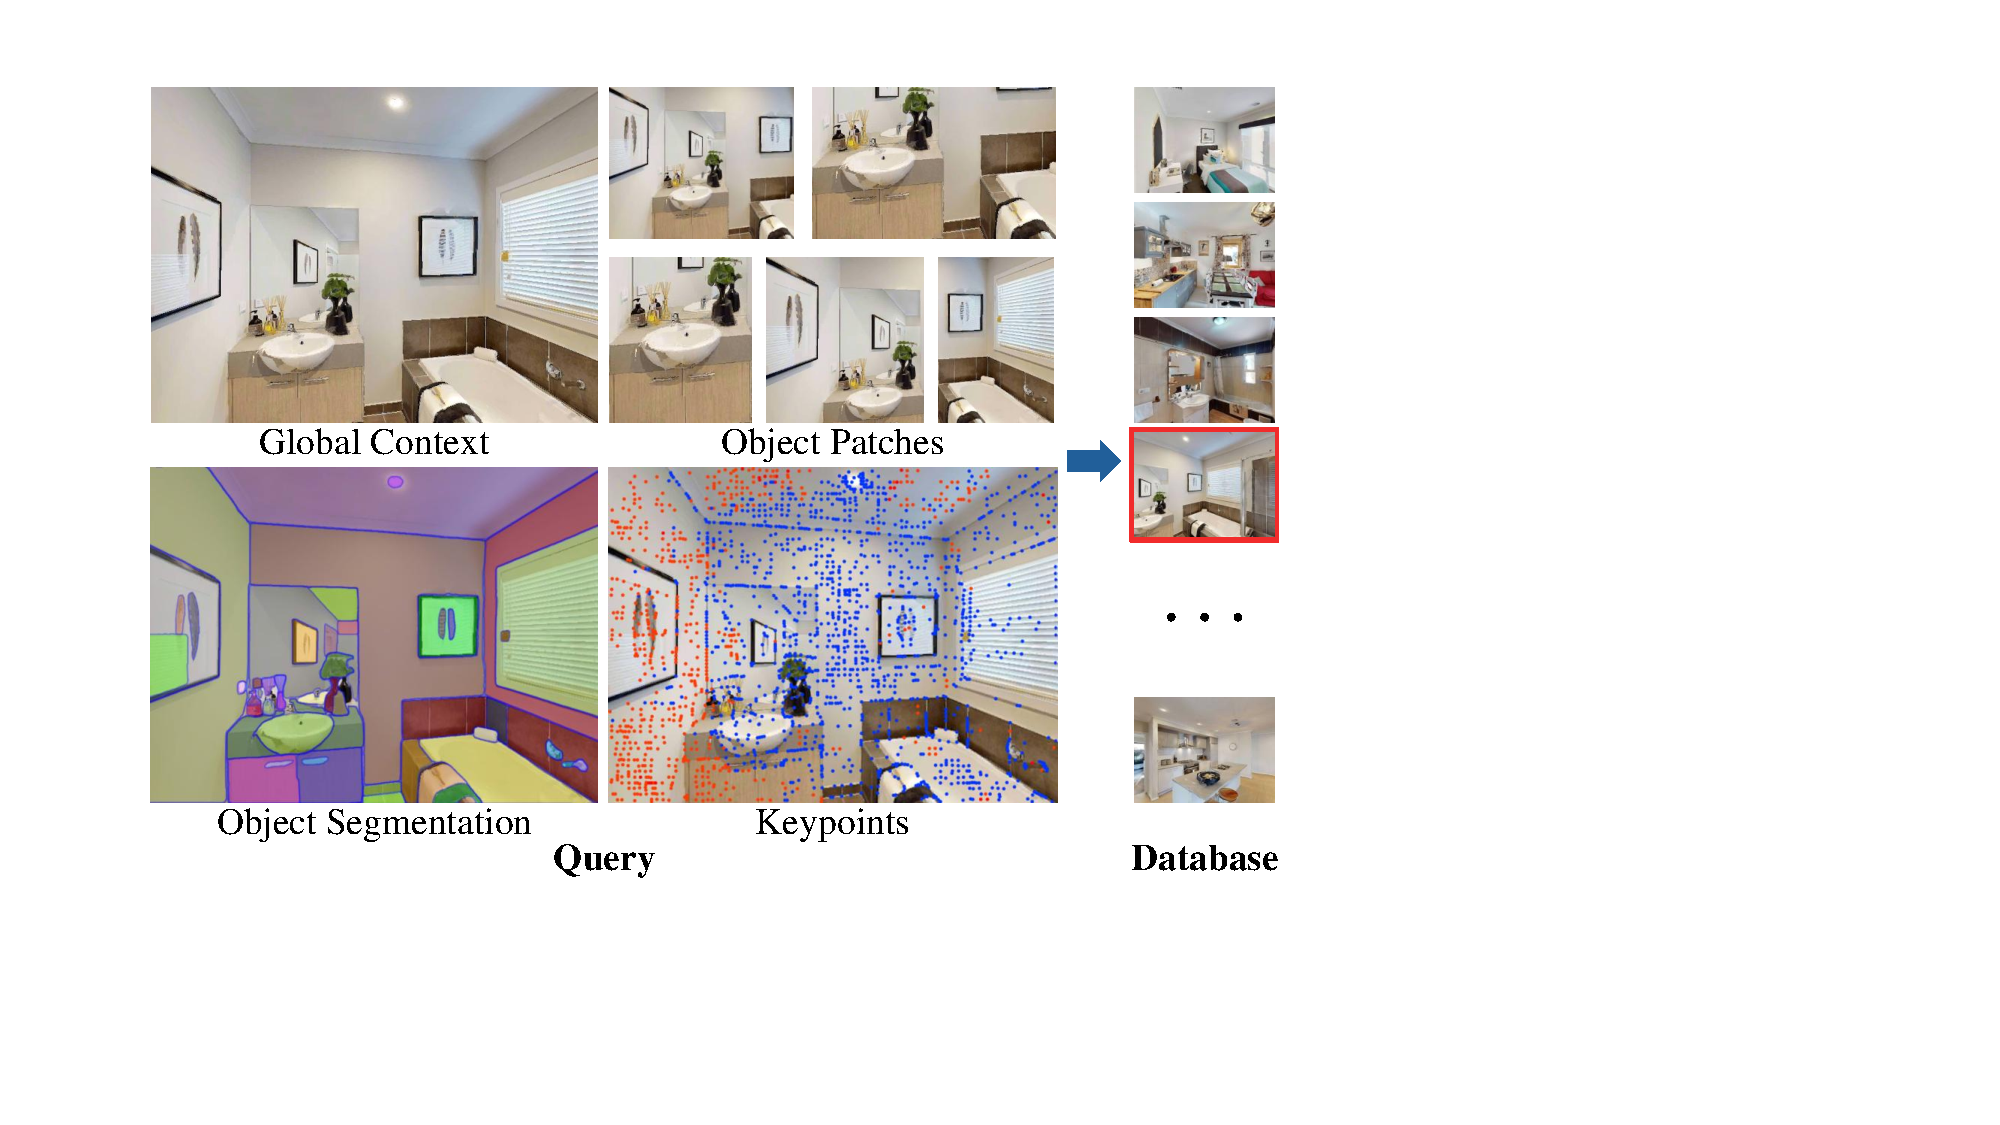
\includegraphics[width=\columnwidth]{object_information_font.pdf}
    \vspace{-20pt}
    \caption{AirRoom leverages multi-level, object-oriented features, including global context, object patches, object segmentation, and keypoints, to perform coarse-to-fine room reidentification.}
    \vspace{-20pt}
    \label{fig:example_image}
\end{figure}

Unlike outdoor environments, where visual place recognition (VPR) methods have matured and perform reliably \cite{arandjelović2016netvladcnnarchitectureweakly, hausler2021patchnetvladmultiscalefusionlocallyglobal, keetha2023anylocuniversalvisualplace}, indoor room ReID remains a challenging problem. A primary reason for this difficulty is the cluttered nature of indoor scenes, which are often densely packed with man-made objects \cite{xu2023clusvprefficientvisualplace}. These densely distributed objects often pose significant challenges to existing methods, which were originally designed for city-style and distinct structures \cite{7339473}. Consequently, these methods struggle to fully capture the intricate details and varied spatial layouts of indoor environments.
% , leading to limitations in their effectiveness when applied to densely populated indoor spaces.
For instance, foundation models like DINO \cite{caron2021emergingpropertiesselfsupervisedvision} and DINOv2 \cite{oquab2024dinov2learningrobustvisual} can generate global descriptors that capture broad scene-level features. However, these descriptors may struggle in semantically similar environments, such as adjacent rooms with similar layouts or decorations, where distinguishable features are minimal \cite{cai2022patchnetvladlearnedpatchdescriptor}. In contrast, methods like Patch-NetVLAD \cite{hausler2021patchnetvladmultiscalefusionlocallyglobal}, AirLoc \cite{aryan2023airlocobjectbasedindoorrelocalization} and AnyLoc \cite{keetha2023anylocuniversalvisualplace} create a global descriptor by aggregating local features, which can enhance discriminative power. Yet, in indoor settings densely populated with similar and repetitive objects, these approaches may still face difficulties in distinguishing between highly similar features, reducing their effectiveness in such contexts \cite{sattler2019understandinglimitationscnnbasedabsolute}.

Additionally, different from room categorization \cite{lee2017roomnetendtoendroomlayout}, which relies on identifying object types to classify spaces into semantic categories, 
%room ReID requires accurately matching specific room instances within a large pre-collected database.
room ReID requires accurately retrieving the same room instance from a reference database based on a given query image. 
For instance, reidentifying a particular kitchen demands a combination of global functional contexts and fine-grained matching of specific object attributes. Moreover, room ReID must handle viewpoint variations, which necessitates tolerance for partial mismatches in object arrangement and appearance. These requirements often result in the failure of algorithms based solely on object categorization, as they lack the precision needed to reidentify unique room instances accurately \cite{Snderhauf2015PlaceRW}.

This raises an important question: \textit{“What kinds of object attributes are truly essential for room ReID?”} To address this, we conduct the first comprehensive study exploring multi-level object-oriented information and its impact on room ReID.
As shown in \fref{fig:example_image}, our experiments show that all four levels of object-oriented information, \ie, global context, object patches, object segmentation, and keypoints, are essential.
Specifically, we find that each level plays a unique role in room ReID. Global context, such as the combination of objects like a couch and television, conveys essential semantic information for categorizing a room as a living room. Object patches provide finer details, enabling differentiation within a room, such as distinguishing a bedside table in a bedroom from a desk in a workspace. Object segmentation offers further granularity by isolating individual items, like separating a dining table from surrounding chairs to clarify the room layout. Finally, keypoints on objects, such as handles on a dresser, enhance room ReID by filtering out visually similar furniture in other rooms. Moreover, integrating multi-level object-oriented information adds robustness to viewpoint variations.

%To address this, we conduct the first comprehensive study that explores the impact of multi-level object information on room ReID. As shown in \fref{fig:example_image}, our experiments demonstrate that all four levels of object information, \textit{i.e.}, global context, object patches, object segmentation, and local keypoints, are essential. Specifically, we find that each level plays a unique role in room ReID. Global context, such as the combination of objects like a couch and television, provides semantic cues to classify a room as a living room. Object patches offer finer detail, helping to distinguish functional zones within a room, such as a sleeping area with a bed and nightstand or a makeup area with a mirror and dressing table in a bedroom. Object segmentation clarifies room layout by isolating specific items, like separating a dining table from surrounding chairs. Finally, local keypoints aid in identifying rooms by filtering out visually similar furniture in other spaces. Moreover, the integration of these four levels of object information significantly improves robustness to viewpoint variations, making our approach adaptable to diverse room perspectives.

% Recent approaches, such as AirLoc \cite{aryan2023airlocobjectbasedindoorrelocalization}, have begun to incorporate object information. However, they rely on pixel-aggregation to form object and room features, which sacrifices critical semantic information, resulting in suboptimal performance. Our findings indicate that objects within indoor environments inherently convey semantic information that aids in room categorization. For example, a combination of objects like a bed, bedside table, and dressing table strongly suggests a bedroom, rather than a kitchen. By incorporating global room representations enriched with object-derived semantics, we achieve broad categorization of rooms. Further, subsets of objects within a room can provide finer details, such as dividing a bedroom into zones like a rest area, with a bed and bedside table, and a makeup area, with a mirror and dressing table. These subsets, or “patches” in image terms, facilitate fine-grained candidate selection. Additionally, individual object details provide further refinement, and local feature matching enhances candidate filtering at an even finer level. Building on these insights, we propose AirRoom—a flexible, object-aware pipeline for room reidentification. AirRoom effectively leverages multi-level object information, boosting reidentification performance while adapting to various configurations, showcasing robustness and versatility across diverse scenarios.

% We find that indoor environments can be broadly categorized into functional types, such as offices, lobbies, and kitchens, each containing distinct semantic information due to the variety of objects present. 
% Global features, rich in appearance and semantic content and extracted from visual backbones, can help select a few functionally similar candidates from a larger pool of irrelevant options \cite{song2022supergfunifyinglocalglobal}. 
% Furthermore, even functionally similar rooms often contain varied objects; for example, different bathrooms may have unique sinks or bathtubs.
% Algorithms that capture this object-level information are generally more effective for achieving accurate and reliable indoor relocalization \cite{qiao2022objectsmatterlearningobject}. 
% Additionally, local feature matching methods, which preserve fine grid information, prove to be highly beneficial \cite{kuang2022densegapgraphstructureddensecorrespondence, wang2024efficientloftrsemidenselocal}. Building on these insights, we propose AirRoom, a novel and flexible object-aware pipeline for indoor relocalization. This approach effectively utilizes object encoding to enhance performance while adapting seamlessly to different module configurations, demonstrating robustness and versatility.
% Recently, methods like AirLoc \cite{aryan2023airlocobjectbasedindoorrelocalization} have attempted to incorporate object information; however, they typically derive object features through a pixel-aggregation approach. This emphasis on local rather than true object-level features has led to limited performance improvements.

% To address these limitations, we pose the question: \textbf{“What if we integrate object encoding into VPR methods?”} We find that indoor environments can be broadly categorized into functional types, such as offices, lobbies, and kitchens, each containing distinct semantic information due to the variety of objects present. Global features, rich in appearance and semantic content and extracted from visual backbones, can help select a few functionally similar candidates from a larger pool of irrelevant options \cite{song2022supergfunifyinglocalglobal}. Furthermore, even functionally similar rooms often contain varied objects; for example, different bathrooms may have unique sinks or bathtubs. Algorithms that capture this object-level information are generally more effective for achieving accurate and reliable indoor relocalization \cite{qiao2022objectsmatterlearningobject}. Additionally, local feature matching methods, which preserve fine grid information, prove to be highly beneficial \cite{kuang2022densegapgraphstructureddensecorrespondence, wang2024efficientloftrsemidenselocal}. Building on these insights, we propose ObjLoc, a novel and flexible object-aware pipeline for indoor relocalization. This approach effectively utilizes object encoding to enhance performance while adapting seamlessly to different module configurations, demonstrating robustness and versatility.
% Recently, methods like AirLoc \cite{aryan2023airlocobjectbasedindoorrelocalization} have attempted to incorporate object information; however, they typically derive object features through a pixel-aggregation approach. This emphasis on local rather than true object-level features has led to limited performance improvements.

Based on these observations, we propose AirRoom, a simple yet highly effective room reidentification (ReID) system consisting of three stages: Global, Local, and Fine-Grained. In the Global stage, a Global Feature Extractor is used to capture global context features, which are then employed to coarsely select five functionally similar candidate rooms. In the Local stage, instance segmentation is applied to identify individual objects, followed by the Receptive Field Expander to extract object patches. An Object Feature Extractor is then used to obtain both object and patch features, which are utilized in Object-Aware Scoring to narrow the selection down to two candidate rooms. Finally, in the Fine-Grained stage, feature matching is employed to precisely identify the final room.

In summary, our contributions include:

\begin{itemize}[leftmargin=2em]
    \item We introduce AirRoom, an object-aware room ReID pipeline with two novel modules: the Receptive Field Expander and Object-Aware Scoring, effectively leveraging multi-level object-oriented information to overcome the limitations observed in previous methods.
    \item We have curated four comprehensive room reidentification datasets—MPReID, HMReID, GibsonReID, and ReplicaReID—providing diverse benchmarks for evaluating room reidentification methods.
    \item Extensive experiments demonstrate that AirRoom outperforms SOTAs, maintaining robust and reliable performance even under significant viewpoint variations.
\end{itemize}

\section{Related Work}
\label{sec:related_work}

In this section, we review areas mostly related to our work, \ie, image retrieval and visual place recognition.

\subsection{Image Retrieval}

Image retrieval is a fundamental and well-established task in computer vision that involves searching for images similar to a given query within a large database.
The process of image retrieval typically consists of two stages: global retrieval and re-ranking. In the first stage, a global descriptor that aggregates local features is used to retrieve $k$ candidates from a large database. This is followed by spatial verification through local feature matching to re-rank these $k$ candidates. Early research relied on handcrafted features \cite{Lowe2004DistinctiveIF, BAY2008346}, while current methods utilize deep networks to learn informative representations \cite{cao2020unifyingdeeplocalglobal, radenović2018finetuningcnnimageretrieval}.

Most image retrieval methods focus on selecting diverse relevant images to help users discover options that align with their interests or needs in real-world applications \cite{Wan2014DeepLF}. Although these methods are effective in retrieving similar images, they often lack the emphasis on distinguishing between categories or achieving precise ReID \cite{10.1145/1348246.1348248}.
In \mbox{contrast}, our approach prioritizes achieving accurate ReID. Following a ``global retrieval and re-ranking" pipeline, we first use global context features to identify the top five room candidates. Our object-aware mechanism then refines the search in a coarse-to-fine manner, progressively distinguishing among candidates until the most similar room is \mbox{identified}, yielding accurate results.

\begin{figure*}[ht]
    \centering
    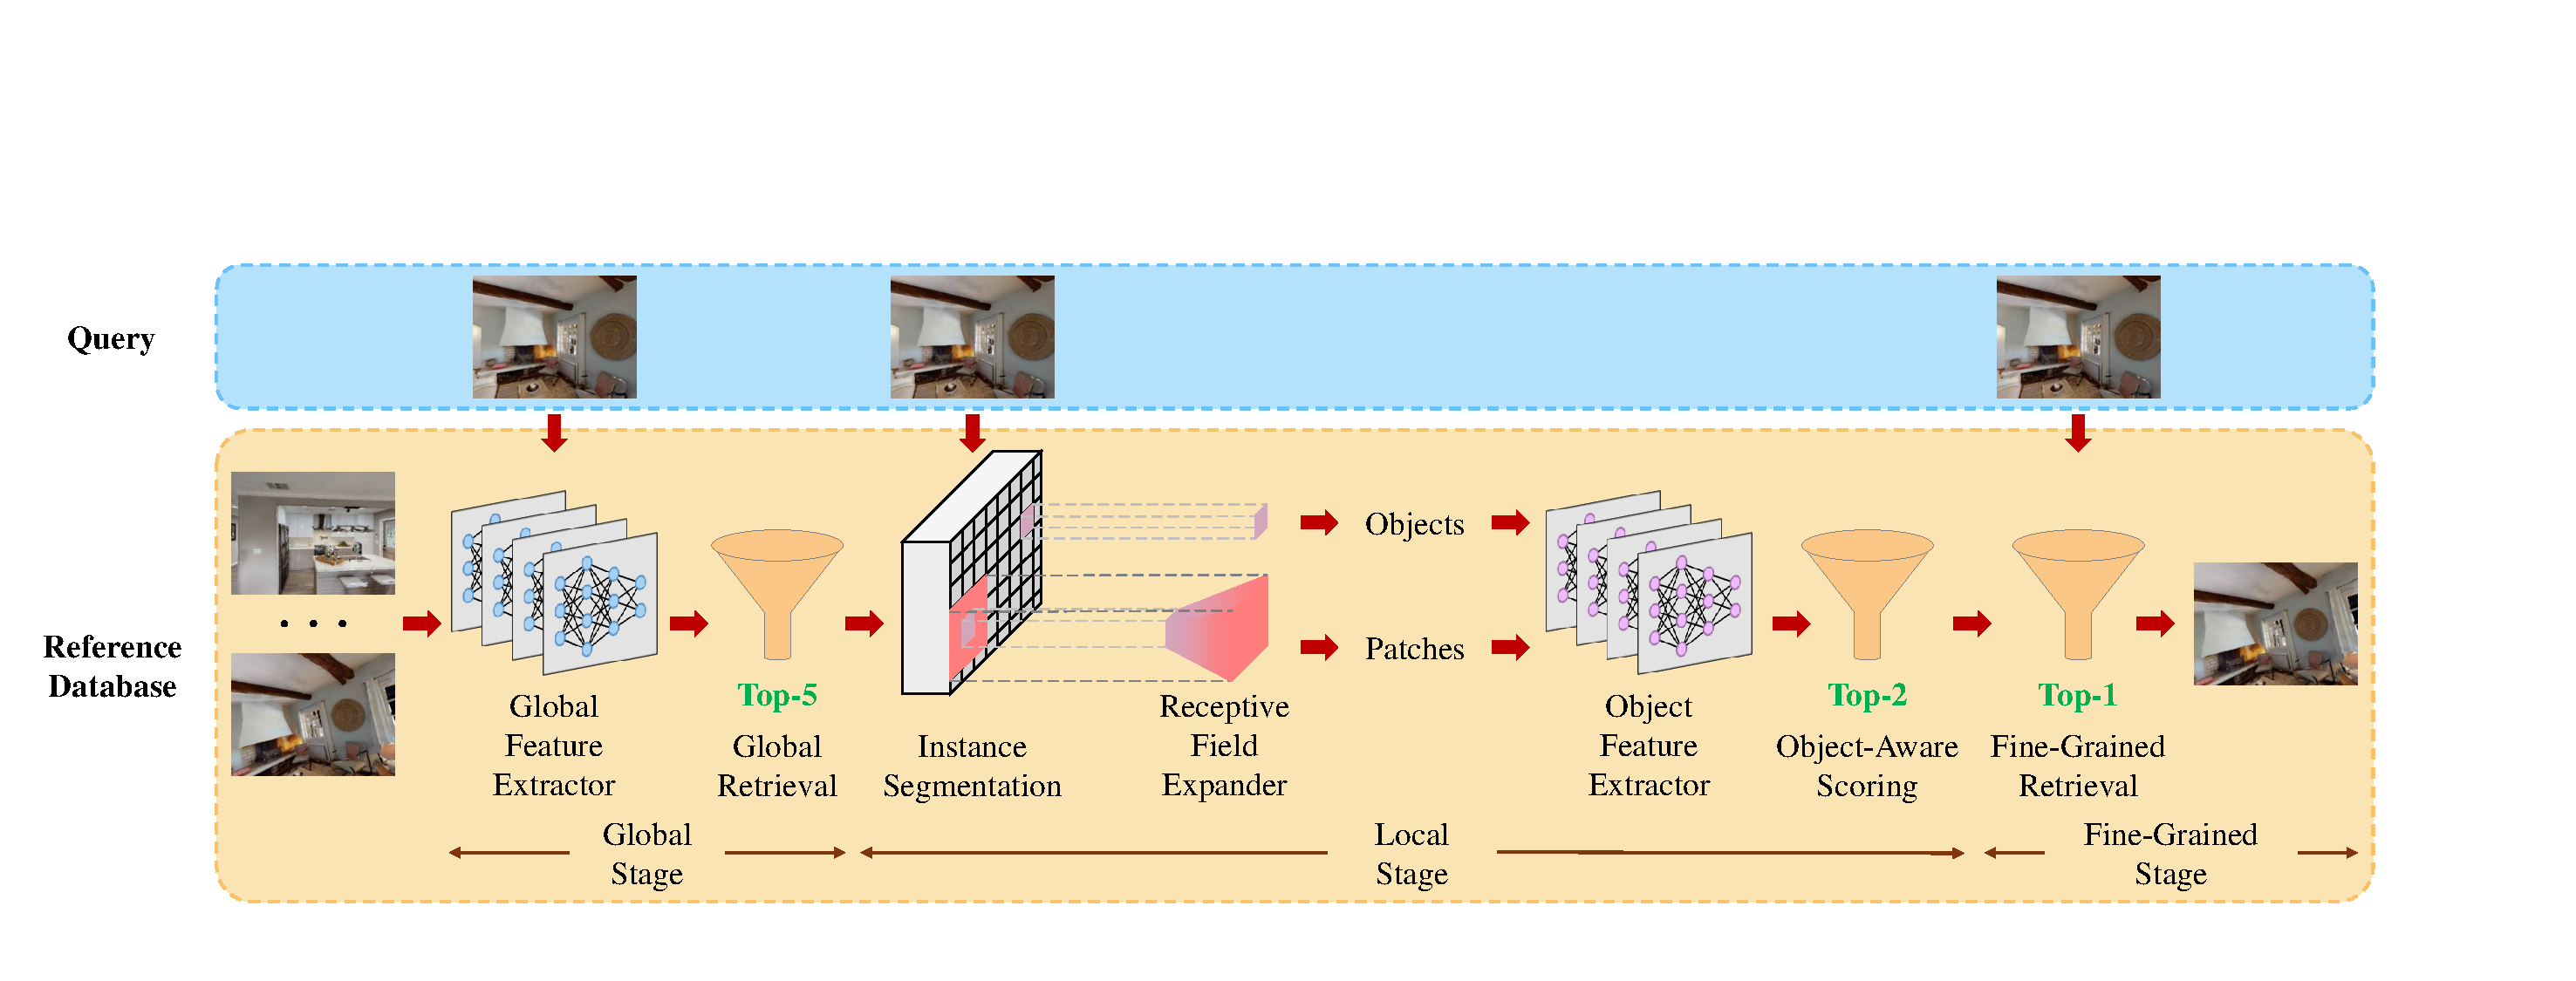
\includegraphics[width=\textwidth]{pipeline_font.pdf}
    \vspace{-16pt}
    \caption{\textbf{The AirRoom coarse-to-fine pipeline}. The pipeline begins with the Global Feature Extractor, which captures global context features to retrieve the top-5 reference images. Instance segmentation then generates object masks, followed by the Receptive Field Expander, which extracts object patches. The Object Feature Extractor processes both object and patch features. The Object-Aware Scoring module narrows the selection to the top-2 candidates, and Fine-Grained Retrieval identifies the most suitable reference image.}
    \vspace{-15pt}
    \label{fig:pipeline}
\end{figure*}

\subsection{Visual Place Recognition}

Visual place recognition (VPR) is often framed as a special image retrieval problem, aiming to match a view of a location with an image of the same place taken under different conditions.
Previous methods fall into two categories: those that directly use global descriptors and those that aggregate local features into a global descriptor. Earlier approaches that relied on global descriptors primarily used CNN-based backbones, such as ResNet \cite{he2015deepresiduallearningimage}, to generate these descriptors. More recent methods, however, leverage foundation models like DINOv2 \cite{oquab2024dinov2learningrobustvisual} for enhanced feature representation. In the aggregation category, early techniques employed handcrafted features like SIFT \cite{Lowe2004DistinctiveIF}, SURF \cite{10.1007/11744023_32}, and ORB \cite{6126544}. Later advancements, including the NetVLAD series \cite{arandjelović2016netvladcnnarchitectureweakly, hausler2021patchnetvladmultiscalefusionlocallyglobal} and AnyLoc \cite{keetha2023anylocuniversalvisualplace}, adopted learning-based models to extract feature maps and combine local features into comprehensive global descriptors.

However, the high performance of most VPR approaches is largely attributed to large-scale training on VPR-specific datasets \cite{keetha2023anylocuniversalvisualplace}. Collecting extensive data for outdoor scenes is relatively straightforward due to natural variations in daylight, weather, and seasons. However, such data collection is more challenging in indoor rooms, making large-scale training on indoor datasets difficult and potentially limiting their effectiveness.
Our approach effectively tackles this challenge by focusing on object-oriented feature representations, allowing us to leverage mature, pre-trained models for object feature learning. This design enables AirRoom to deliver robust performance without requiring any additional training or fine-tuning on specific datasets.
% Our approach addresses this challenge by centering on objects within indoor spaces, leveraging object-related feature representations. Additionally, AirRoom benefits from mature, pre-trained models for object-centric feature learning. This design enables our approach to deliver robust performance without the need for additional training or fine-tuning on specific datasets.
\section{Proposed Approach}
\label{sec:proposed_approach}

We propose a simple yet highly effective pipeline, AirRoom, for room reidentification that leverages multi-level object-oriented information, as shown in \fref{fig:pipeline}. We will now systematically introduce each module of the pipeline, following the sequence of stages in which they are executed.

\subsection{Global Stage}

In this stage, we utilize the Global Feature Extractor to capture global context features, which are derived from the collective presence of objects within the room. These features are then used for Global Retrieval, coarsely selecting semantically similar candidate rooms from the database.

\subsubsection{Global Feature Extractor}
\label{sec:section3.1.1}

Indoor rooms exhibit fewer variations compared to outdoor environments. They lack diverse topographies, such as aerial, subterranean, or underwater features, and do not experience temporal changes like day-night or seasonal variations. Consequently, collecting large datasets for each indoor room is challenging, complicating large-scale training as seen in many VPR methods \cite{arandjelović2016netvladcnnarchitectureweakly, hausler2021patchnetvladmultiscalefusionlocallyglobal, alibey2023mixvprfeaturemixingvisual}. 

However, indoor rooms are inherently rich in objects, each contributing to the room’s overall semantic context. By leveraging this global context information, we can refine the reference search to specifically focus on rooms with similar semantic features to those in the query image. For this purpose, we prefer backbones pretrained on large image datasets, as they provide strong generalizability and effectively capture informative global context features \cite{kornblith2019betterimagenetmodelstransfer}. Our model selections, therefore, include pretrained CNN-based models such as ResNet \cite{he2015deepresiduallearningimage} and transformer-based self-supervised models like DINOv2 \cite{oquab2024dinov2learningrobustvisual}.

\subsubsection{Global Retrieval}

Using the Global Feature Extractor, we extract global context features for \(M\) query and \(N\) reference images. Let \(\mathbf{Q} \in \mathbb{R}^{M \times D_g}\) and \(\mathbf{R} \in \mathbb{R}^{N \times D_g}\) denote the query and reference features, respectively, where \(D_g\) is the feature dimension. The cosine similarity matrix \(\mathbf{S}\) is then computed as:
% Using the Global Feature Extractor, we first extract global context features for \(M\) query and \(N\) reference images. Given \(M\) query features \(\mathbf{Q} \in \mathbb{R}^{M \times D_g}\) and \(N\) reference features \(\mathbf{R} \in \mathbb{R}^{N \times D_g}\), where \(D_g\) denotes the global context feature dimension, we have a cosine similarity matrix \(\mathbf{S}\):
\begin{equation}
    \mathbf{S}_{ij} = \frac{\mathbf{Q}_i \cdot \mathbf{R}_j}{\|\mathbf{Q}_i\| \|\mathbf{R}_j\|}.
    \label{eq:global feature cosine similarity}
\end{equation}
For each query, we select the top-5 most similar reference candidates using the following formula:
\begin{equation}
    \text{Top}_5(\mathbf{S}_{i, :}) = \text{argsort}(-\mathbf{S}_{i, :})[:5],
    \label{eq:global retrieval}
\end{equation}
where \(\mathbf{S}_{i, :}\) represents the cosine similarity for the \(i\)-th query.

\subsection{Local Stage}

Global context features provide valuable semantic information that helps narrow down the candidate list. However, when faced with many semantically similar rooms, relying solely on global context is insufficient, and local features become increasingly essential. In this stage, we adopt a local perspective by first applying instance segmentation and the Receptive Field Expander to identify objects and patches. We then use the Object Feature Extractor to extract features from both objects and patches, followed by Object-Aware Scoring to further refine the candidate list.

\subsubsection{Instance Segmentation}

For each query image and its corresponding five candidates, we employ instance segmentation methods, such as Mask R-CNN \cite{he2018maskrcnn} and Semantic-SAM \cite{li2023semanticsamsegmentrecognizegranularity}, to identify and delineate individual objects. This process generates each object's mask and bounding box. Next, we calculate the center point \(c\) of each object using its bounding box, as shown below:

\begin{equation}
    c = (\frac{x+W}{2}, \frac{y+H}{2}).
    \label{eq:center point}
\end{equation}
In this equation, \(x\) and \(y\) represent the pixel coordinates of the top-left corner of the bounding box, while \(W\) and \(H\) denote the width and height of the bounding box, respectively.

\subsubsection{Receptive Field Expander}

Single object information alone is not sufficiently discriminative. For example, although different desks may have distinct appearances, they can be found in both dining halls and offices. However, when an object is connected with its neighboring items—such as a desk alongside a computer, keyboard, or notebook—it suggests that the room is more likely to be an office rather than a dining hall. This insight motivates us to expand the receptive field from a single object to a patch containing multiple objects.

Given the center points of all objects in an image, we employ Delaunay triangulation \cite{10.5555/1370949} to generate a triangulated graph of object relationships. Specifically, Delaunay triangulation is applied to the set of object centers, ensuring that no object centers are inside the circumcircle of any triangle. This method maximizes the minimum angle of the triangles, preventing narrow, elongated triangles and ensuring more uniform object adjacency. By analyzing the adjacency relationships among the resulting triangles, we can construct the object adjacency matrix, which encodes the spatial and relational proximity of objects within the room.

\vspace{-10pt}
\begin{figure}[ht]
    \centering
    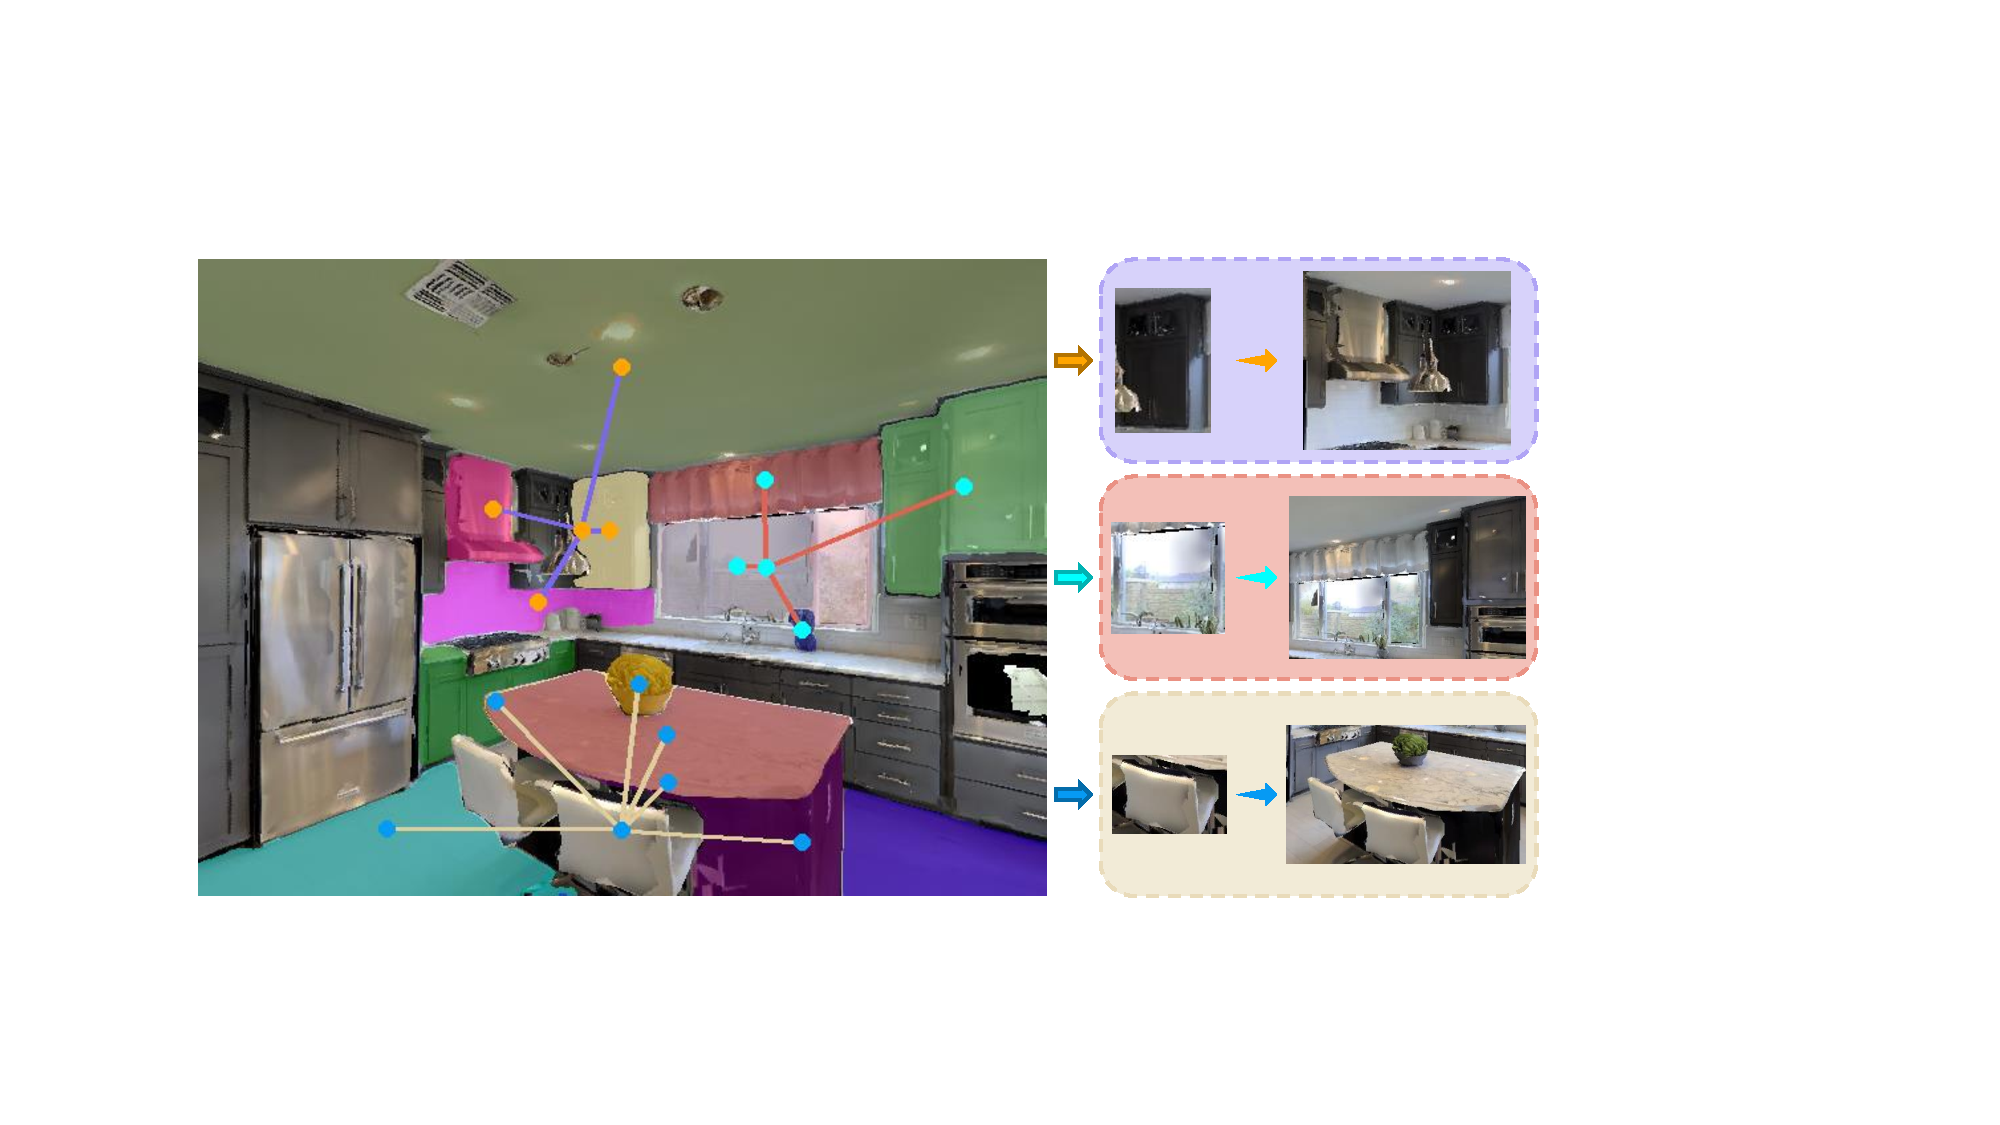
\includegraphics[width=\columnwidth]{expander.pdf}
    \vspace{-20pt}
    \caption{The Receptive Field Expander broadens the receptive field from individual objects to patches rich in contextual information. Leveraging the object adjacency matrix and each object's bounding box, it expands single objects such as a cupboard, window pane, and chair into object patches like a modular kitchen, multi-pane window, and dining set, respectively.}
    \vspace{-5pt}
    \label{fig:expander_image}
\end{figure}

% Given the center points of all objects in an image, we use Delaunay triangulation to create the object adjacency matrix. This mathematical technique takes a set of discrete points and generates triangles that maximize the minimum angle of each triangle, thus avoiding narrow shapes. A key property of Delaunay triangulation is that no discrete point lies within the circumcircle of any triangle formed in the process. By analyzing the adjacency relationships of the triangles created through Delaunay triangulation, we can construct the object adjacency matrix.

Given the object adjacency matrix and bounding boxes in an image, for each object, we consider the bounding boxes of its neighboring objects and enlarge the current object's bounding box to encompass all adjacent objects. This expansion increases the receptive field, enabling us to capture richer contextual information, as illustrated in \fref{fig:expander_image}. We then apply Non-Maximum Suppression (NMS) to select the highest confidence bounding boxes, removing overlapping ones based on their Intersection over Union (IoU) scores. This results in a set of clean, informative object patches.

\begin{figure*}[t]
    \centering
    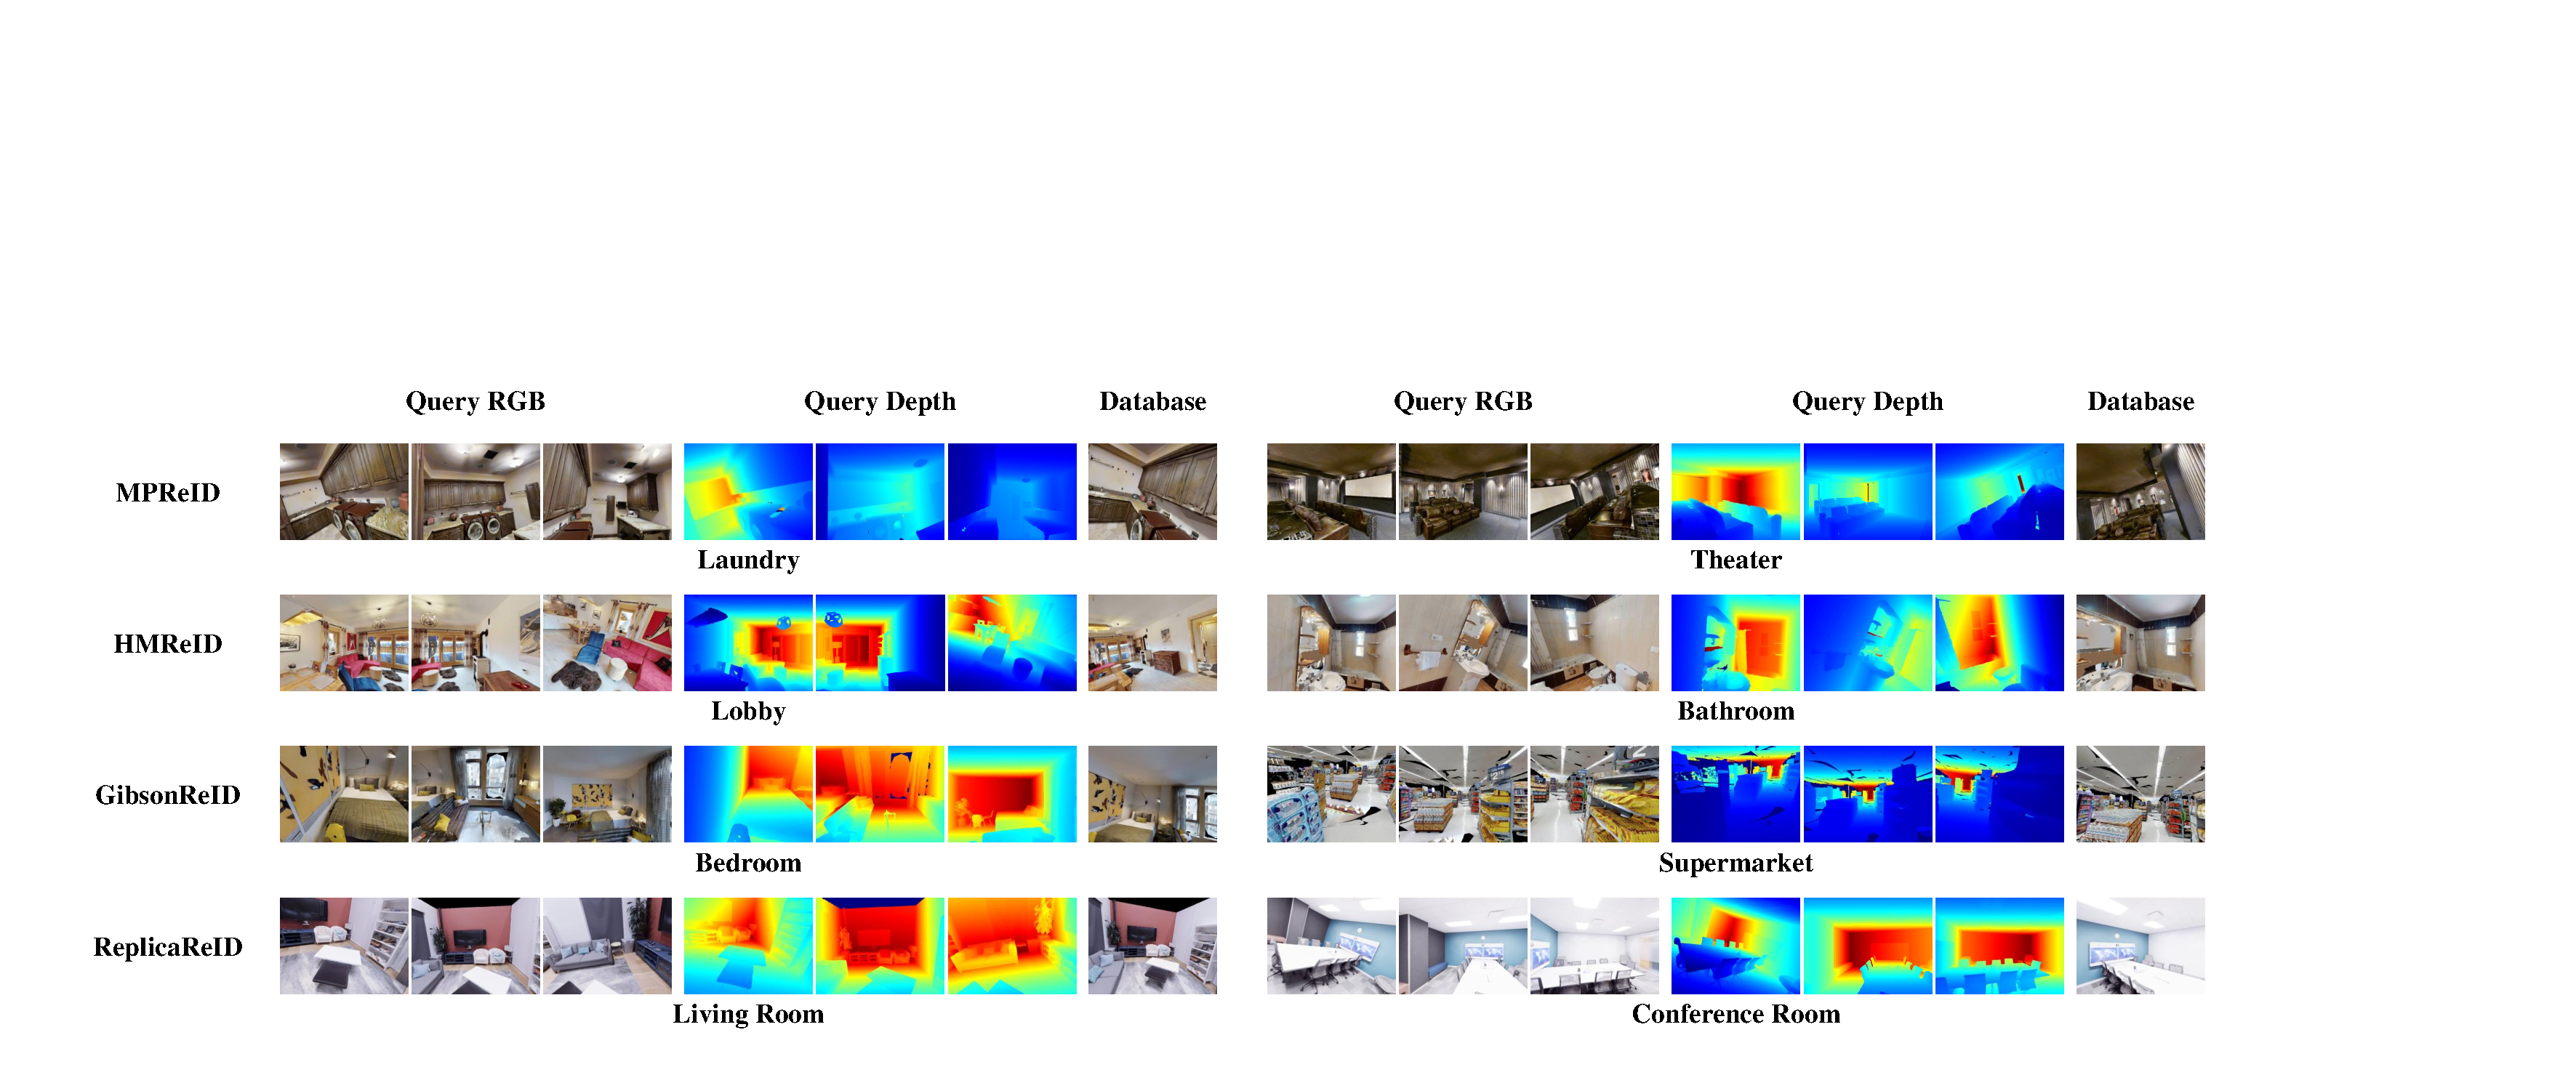
\includegraphics[width=\textwidth]{dataset_font.pdf}
    \vspace{-20pt}
    \caption{Illustration of four newly constructed room reidentification datasets: MPReID, HMReID, GibsonReID, and ReplicaReID. Each room provides only one reference image in the database, while query images for each room capture varied viewpoints.}
    \vspace{-10pt}
    \label{fig:dataset_image}
\end{figure*}

\subsubsection{Object-Aware Refinement}
\label{subsec:refinement}

The Object-Aware Refinement module is composed of three key submodules: Object Feature Extractor, Mutual Nearest Neighbors, and Object-Aware Scoring.

\vspace{-6pt}
\paragraph{Object Feature Extractor}

To effectively leverage object patches and object segmentation information, we prioritize global features over local feature aggregation. The latter approach may fail to capture object characteristics effectively and can significantly increase computational complexity and storage demands \cite{zheng2018sift}. As discussed in Section~\ref{sec:section3.1.1}, we continue to rely on models pre-trained on large image datasets. Using the Object Feature Extractor, we obtain features for both query and reference patches and objects. Let \(Q_p=\{\mathbf{p_i^q}\}_{i=1}^{n_{qp}}\) and \(Q_o=\{\mathbf{o_i^q}\}_{i=1}^{n_{qo}}\) represent the query patch and object feature sets, respectively. For each reference image among the query’s five \mbox{candidates}, we define the reference patch and object feature sets as \(R_p=\{\mathbf{p_i^r}\}_{i=1}^{n_{rp}}\) and \(R_o=\{\mathbf{o_i^r}\}_{i=1}^{n_{ro}}\).

\vspace{-6pt}
\paragraph{Mutual Nearest Neighbors} Given a set of query features \(\{\mathbf{f_i^q}\}_{i=1}^{n_q}\) and reference features \(\{\mathbf{f_i^r}\}_{i=1}^{n_r}\), we obtain feature pairs by identifying mutual nearest neighbor matches through exhaustive comparison of the two sets. Let \(P\) denote the set of cosine similarity scores for these mutual nearest neighbor matches, then we have
\begin{equation}
    P = \{\cos(\mathbf{f_i^q}, \mathbf{f_j^r}) \mid i = \text{NN}_r(\mathbf{f_j^r}), \; j = \text{NN}_q(\mathbf{f_i^q})\}
    \label{eq:mutual nearest neighbors}
\end{equation}
where
\begin{equation}
    \text{NN}_q(\mathbf{f_i^q}) = \arg\max_{j} \left( \frac{\mathbf{f_i^q} \cdot \mathbf{f_j^r}}{\|\mathbf{f_i^q}\| \|\mathbf{f_j^r}\|} \right),
\end{equation}
\begin{equation}
    \text{NN}_r(\mathbf{f_i^r}) = \arg\max_{j} \left( \frac{\mathbf{f_i^r} \cdot \mathbf{f_j^q}}{\|\mathbf{f_i^r}\| \|\mathbf{f_j^q}\|} \right),
\end{equation}
\begin{equation}
    \cos(\mathbf{f_i^q}, \mathbf{f_j^r}) = \frac{\mathbf{f_i^q} \cdot \mathbf{f_j^r}}{\|\mathbf{f_i^q}\| \|\mathbf{f_j^r}\|}.
\end{equation}
% By utilizing mutual nearest neighbors, we can improve retrieval accuracy while narrowing the search space and enhancing retrieval efficiency \cite{zhong2017reranking}.
By utilizing mutual nearest neighbors, we can significantly improve retrieval accuracy, simultaneously narrowing the search space and enhancing overall retrieval efficiency \cite{zhong2017reranking}.

\vspace{-6pt}
\paragraph{Object-Aware Scoring} The object-aware score \(s\) is the sum of the global score \(s_{\text{global}}\) (calculated in Equation~\ref{eq:global feature cosine similarity}), the patch score \(s_{\text{patch}}\), and the object score \(s_{\text{object}}\):
\begin{equation}
    s = s_{\text{global}} + s_{\text{patch}}(Q_p, R_p) + s_{\text{object}}(Q_o, R_o).
    \label{eq:object-aware scoring}
\end{equation}
Here, \(s_{\text{patch}}\) and \(s_{\text{object}}\) can either be \(s_{\text{mean}}\) or \(s_{\max}\), where
\begin{subequations}
\begin{align}
    s_{\text{mean}}(Q_t, R_t) &= \frac{1}{|P(Q_t, R_t)|} \sum_{x \in P(Q_t, R_t)} x,
    \label{eq:mean}\\
    s_{\max}(Q_t, R_t) &= \max_{x \in P(Q_t, R_t)} x.
    \label{eq:max}
\end{align}
\end{subequations}
In these equations, \(P\) denotes the set of cosine similarity scores for mutual nearest neighbor matches, with \(Q_t\) representing either \(Q_p\) or \(Q_o\), and \(R_t\) representing either \(R_p\) or \(R_o\). The global score \(s_{\text{global}}\) serves as a prior, indicating that the initial five candidates vary in relevance. Thus, we retain this term to account for their differing levels of relevance.

\vspace{-8pt}
\paragraph{Object-Aware Refinement} For each query, we select the top-2 most similar reference candidates from the initial five using the Object-Aware Scoring:
\begin{equation}
    \text{Top}_2(\mathbf{s}_{i}) = \text{argsort}(-\mathbf{s}_{i})[:2],
\end{equation}
where \(\mathbf{s}_{i}\) is the object-aware scores for the \(i\)-th query.

\subsection{Fine-Grained Stage}

Patch and object features provide valuable information for understanding the room layout; however, they may be insufficient when distinguishing highly visually similar rooms, particularly in the presence of viewpoint variations and occlusions. Keypoints on objects, by contrast, exhibit strong robustness to texture and appearance variations, enabling them to effectively handle partial occlusions and reject outliers \cite{1498756}. This allows keypoints to offer a more refined approach, capturing finer details for more accurate room identification. In this stage, we use Fine-Grained Retrieval to select the final top-1 result.

\subsubsection{Fine-Grained Retrieval}

Deep matchers, such as SuperGlue \cite{sarlin2020supergluelearningfeaturematching}, perform well in visual localization tasks under challenging conditions, both indoors and outdoors. However, they tend to face efficiency issues. In contrast, LightGlue \cite{lindenberger2023lightgluelocalfeaturematching} offers high efficiency without compromising matching accuracy, making it an ideal choice for our Fine-Grained Retrieval.

For each query image and its two candidate reference images, we match the query to each candidate and record the number of matching keypoint pairs. A higher number of matches typically indicates greater overlap and consistency between the features of the two images, suggesting a higher degree of similarity in their content \cite{Lowe2004DistinctiveIF}. The candidate with more matches is selected as the final result.

\vspace{-3pt}
\section{实验结果}
\label{sec:experimental_results}

\begin{table*}[t]
\centering
\resizebox{\textwidth}{!}{
\begin{tabular}{l|cccc|cccc|cccc|cccc}
\toprule
\multirow{2}{*}{\textbf{Methods}} & \multicolumn{4}{c|}{\textbf{MPReID}} & \multicolumn{4}{c|}{\textbf{HMReID}} & \multicolumn{4}{c|}{\textbf{GibsonReID}} & \multicolumn{4}{c}{\textbf{ReplicaReID}} \\
 & Accuracy & Precision & Recall & F1 & Accuracy & Precision & Recall & F1 & Accuracy & Precision & Recall & F1 & Accuracy & Precision & Recall & F1 \\
\midrule
CVNet & 17.45 & 29.52 & 17.45 & 19.34 & 11.71 & 25.42 & 11.95 & 13.86 & 12.04 & 24.06 & 12.07 & 14.27 & 15.93 & 20.53 & 15.74 & 16.64 \\
DINOv2 & 59.36 & 64.68 & 59.36 & 58.91 & 53.91 & 60.52 & 53.73 & 54.69 & 61.01 & 65.88 & 61.78 & 61.71 & 78.06 & 79.68 & 77.97 & 77.44 \\
Patch-NetVLAD & 64.32 & 70.47 & 64.36 & 65.53 & 64.86 & 68.78 & 64.32 & 65.16 & 61.47 & 66.90 & 62.04 & 62.51 & 63.77 & 64.97 & 63.86 & 63.87 \\
AnyLoc & 92.34 & 93.23 & 92.36 & 92.32 & 89.69 & 90.25 & 89.53 & 89.62 & 85.85 & 87.42 & 86.15 & 86.21 & \textbf{88.57} & \textbf{89.89} & \textbf{88.46} & \textbf{88.42} \\
\rowcolor{Lavender}
AirRoom & \textbf{93.96} & \textbf{94.52} & \textbf{93.98} & \textbf{93.91} & \textbf{93.80} & \textbf{94.01} & \textbf{93.55} & \textbf{93.62} & \textbf{91.68} & \textbf{92.41} & \textbf{91.79} & \textbf{91.63} & 87.18 & 89.39 & 87.08 & 87.24 \\
\bottomrule
\end{tabular}
}
\vspace{-5pt}
\caption{AirRoom 与基线模型在四个新构建的房间重识别数据集上的整体性能对比。}
\vspace{-12pt}
\label{tab:overall}
\end{table*}
\subsection{数据集}
\vspace{-5pt}
目前没有现有的室内场景数据集完全适用于房间再识别任务,因为没有一个数据集能完全满足要求。像 ScanNet++ \cite{yeshwanth2023scannethighfidelitydataset3d} 和 MIT Indoor Scenes \cite{5206537} 这样的数据集缺乏房间级别的分割,导致多个房间共享一个场景标签。17 Places \cite{7801503} 数据集包含了唯一标签的房间,但视角变化有限,而且图像往往较为模糊。尽管该数据集也包含昼夜变化,但这些变化对于大多数室内场景并不特别相关。Reloc110 \cite{aryan2023airlocobjectbasedindoorrelocalization} 数据集可能是最合适的选择;然而,它的质量不够理想,许多图像仅包含纯色的墙壁或地板,由于随机采样,导致上下文信息非常少。

一些高质量的室内 3D 数据集——如 Matterport3D \cite{Matterport3D}、Habitat-Matterport3D \cite{ramakrishnan2021hm3d}、Gibson Database of 3D Spaces \cite{xiazamirhe2018gibsonenv} 和 Replica \cite{replica19arxiv}——提供了真实世界的室内场景。基于这些资源,并利用互动式 Habitat Simulator \cite{puig2023habitat3, szot2021habitat, habitat19iccv},我们创建了四个新的数据集:MPReID、HMReID、GibsonReID 和 ReplicaReID,如 \fref{fig:dataset_image} 所示。

使用 Habitat Simulator,我们为每个房间配置了一个代理,并手动选择了 5 到 10 个关键姿势来引导其探索。代理从不同角度捕捉了 640×480 的 RGB-D 图像,每个房间的图像数量为 300 到 800 张,具体取决于关键姿势的数量。然而,许多随机采样的图像质量较差,通常只包含墙壁或地板,缺乏足够的上下文信息。为了解决这一问题,我们仔细筛选了每个房间的图像,保留了那些准确代表空间并为房间 ReID 提供有价值信息的图像。

总的来说,这些数据集如下:MPReID 包括 15 个场景、105 个房间和 16,231 张 RGB-D 图像;HMReID 包含 21 个场景、105 个房间和 15,781 张 RGB-D 图像;GibsonReID 包含 24 个场景、45 个房间和 6,743 张 RGB-D 图像;ReplicaReID 包括 12 个场景、19 个房间和 2,862 张 RGB-D 图像。

\vspace{-4pt}
\subsection{数据库预处理}
\vspace{-4pt}

在房间重识别设置中,我们有多个查询图像和一个参考数据库。对于每个数据集,我们仅选择每个房间的一张图像来构建数据库。具体来说,对于每个房间的所有图像,我们首先使用 CLIP \cite{radford2021learningtransferablevisualmodels} 提取特征嵌入。然后,我们应用 K-means 聚类,设定聚类数为 1。距离聚类中心最近的图像被选择为参考图像,因为它最能代表房间的视觉特征 \cite{tan2005introduction}。

在构建参考数据库后,我们对特征进行预处理。首先,我们使用全局特征提取器来获取并保存全局上下文特征。接着,我们应用实例分割模块对物体进行分割。然后,我们使用我们的感受野扩展器来获取物体补丁,并使用物体特征提取器来提取并保存物体和补丁的特征。

\vspace{-4pt}
\subsection{实验概述}
\vspace{-4pt}
我们进行了五个主要实验:整体性能比较、分组性能比较、管道灵活性评估、消融研究和运行时分析。在评估过程中,我们使用了准确率、精确度、召回率和F1分数作为评价指标。每个类别的精确度、召回率和F1分数是通过多类混淆矩阵计算得出的,随后进行了宏平均。准确率是通过正确匹配的查询与总查询数之比来衡量的。详细的运行时分析和其他实验结果在附录中提供。

\begin{table*}[t]
\centering
\resizebox{\textwidth}{!}{
\begin{tabular}{l|cccc|cccc|cccc|cccc}
\toprule
\multirow{2}{*}{\textbf{Methods}} & \multicolumn{4}{c|}{\textbf{MPReID}} & \multicolumn{4}{c|}{\textbf{HMReID}} & \multicolumn{4}{c|}{\textbf{GibsonReID}} & \multicolumn{4}{c}{\textbf{ReplicaReID}} \\
 & Accuracy & Precision & Recall & F1 & Accuracy & Precision & Recall & F1 & Accuracy & Precision & Recall & F1 & Accuracy & Precision & Recall & F1 \\
\midrule
ResNet50 & 76.14 & 79.21 & 76.20 & 76.58 & 69.03 & 73.21 & 68.61 & 69.07 & 68.84 & 72.30 & 69.50 & 69.00 & 75.05 & 78.61 & 75.30 & 74.88 \\
CVNet & 17.45 & 29.52 & 17.45 & 19.34 & 11.71 & 25.42 & 11.95 & 13.86 & 12.04 & 24.06 & 12.07 & 14.27 & 15.93 & 20.53 & 15.74 & 16.64 \\
\rowcolor{Lavender}
AirRoom-ResNet50 & \textbf{86.16} & \textbf{87.69} & \textbf{86.19} & \textbf{86.16} & \textbf{81.23} & \textbf{83.90} & \textbf{80.76} & \textbf{81.23} & \textbf{82.53} & \textbf{84.91} & \textbf{82.86} & \textbf{82.54} & \textbf{83.51} & \textbf{84.85} & \textbf{83.54} & \textbf{83.17} \\
\cdashline{1-17}
NetVLAD & 82.22 & 86.77 & 82.24 & 82.92 & 72.04 & 80.79 & 71.83 & 73.05 & 68.86 & 81.00 & 69.24 & 71.01 & 77.04 & 81.31 & 77.28 & 77.63 \\
Patch-NetVLAD(4096) & 64.32 & 70.47 & 64.36 & 65.53 & 64.86 & 68.78 & 64.32 & 65.16 & 61.47 & 66.90 & 62.04 & 62.51 & 63.77 & 64.97 & 63.86 & 63.87 \\
Patch-NetVLAD(512) & 66.62 & 71.85 & 66.67 & 67.62 & 65.63 & 69.28 & 65.01 & 65.57 & 60.95 & 69.16 & 61.43 & 62.46 & 66.00 & 68.75 & 66.25 & 66.22 \\
Patch-NetVLAD(128) & 65.04 & 70.84 & 65.09 & 66.15 & 61.17 & 66.71 & 60.69 & 61.42 & 58.31 & 66.15 & 58.69 & 59.66 & 61.88 & 66.29 & 62.12 & 62.05 \\
\rowcolor{Lavender}
AirRoom-NetVLAD & \textbf{89.38} & \textbf{90.99} & \textbf{89.40} & \textbf{89.50} & \textbf{83.47} & \textbf{86.91} & \textbf{83.08} & \textbf{83.66} & \textbf{82.29} & \textbf{87.27} & \textbf{82.61} & \textbf{82.98} & \textbf{83.58} & \textbf{84.42} & \textbf{83.60} & \textbf{83.37} \\
\bottomrule
\end{tabular}
}
\vspace{-6pt}
\caption{与基准模型的组别性能比较,以评估面向对象机制的有效性。}
\vspace{-5pt}
\label{tab:grouped}
\end{table*}

\begin{table*}[t]
\centering
\resizebox{\textwidth}{!}{
\begin{tabular}{l|cccc|cccc|cccc|cccc}
\toprule
\multirow{2}{*}{\textbf{Methods}} & \multicolumn{4}{c|}{\textbf{MPReID}} & \multicolumn{4}{c|}{\textbf{HMReID}} & \multicolumn{4}{c|}{\textbf{GibsonReID}} & \multicolumn{4}{c}{\textbf{ReplicaReID}} \\
 & Accuracy & Precision & Recall & F1 & Accuracy & Precision & Recall & F1 & Accuracy & Precision & Recall & F1 & Accuracy & Precision & Recall & F1 \\
\midrule
ViT & 81.90 & 85.27 & 81.96 & 81.71 & 76.47 & 79.37 & 76.04 & 75.91 & 76.46 & 78.51 & 77.00 & 76.88 & 77.99 & 81.41 & 78.15 & 77.46 \\
\rowcolor{Lavender} AirRoom-ViT & \textbf{89.70} & \textbf{90.97} & \textbf{89.72} & \textbf{89.35} & \textbf{86.58} & \textbf{88.13} & \textbf{86.12} & \textbf{86.23} & \textbf{87.08} & \textbf{88.24} & \textbf{87.33} & \textbf{87.19} & \textbf{84.84} & \textbf{86.85} & \textbf{84.79} & \textbf{84.45} \\
\cdashline{1-17}
DINO & 80.66 & 84.32 & 80.73 & 81.14 & 73.54 & 77.73 & 73.13 & 73.79 & 72.28 & 74.92 & 72.92 & 72.89 & 86.58 & 87.77 & 86.60 & 86.49 \\
\rowcolor{Lavender} AirRoom-DINO & \textbf{88.00} & \textbf{89.59} & \textbf{88.05} & \textbf{88.09} & \textbf{83.62} & \textbf{85.43} & \textbf{83.14} & \textbf{83.40} & \textbf{84.62} & \textbf{86.23} & \textbf{84.95} & \textbf{84.83} & \textbf{87.49} & \textbf{88.56} & \textbf{87.41} & \textbf{87.25} \\
\cdashline{1-17}
DINOv2 & 59.36 & 64.68 & 59.36 & 58.91 & 53.91 & 60.52 & 53.73 & 54.69 & 61.01 & 65.88 & 61.78 & 61.71 & 78.06 & 79.68 & 77.97 & 77.44 \\
\rowcolor{Lavender} AirRoom-DINOv2 & \textbf{76.10} & \textbf{79.03} & \textbf{76.11} & \textbf{75.80} & \textbf{70.95} & \textbf{73.86} & \textbf{70.66} & \textbf{70.78} & \textbf{78.63} & \textbf{80.44} & \textbf{79.00} & \textbf{78.45} & \textbf{85.57} & \textbf{86.58} & \textbf{85.45} & \textbf{85.19} \\
\cdashline{1-17}
AnyLoc(16) & 90.22 & 91.18 & 90.25 & 90.17 & 84.63 & 86.40 & 84.56 & 84.91 & 82.20 & 83.77 & 82.59 & 82.74 & 85.64 & 87.52 & 85.59 & 85.67 \\
\rowcolor{Lavender} AirRoom-AnyLoc(16) & \textbf{93.05} & \textbf{93.66} & \textbf{93.08} & \textbf{92.99} & \textbf{91.55} & \textbf{92.12} & \textbf{91.32} & \textbf{91.47} & \textbf{89.04} & \textbf{89.97} & \textbf{89.21} & \textbf{89.13} & \textbf{86.83} & \textbf{89.03} & \textbf{86.76} & \textbf{86.90} \\
\cdashline{1-17}
AnyLoc(8) & 88.03 & 89.33 & 88.08 & 88.01 & 81.93 & 83.89 & 81.94 & 82.25 & 79.27 & 81.29 & 79.72 & 79.71 & 84.98 & 86.19 & 85.03 & 84.88 \\
\rowcolor{Lavender} AirRoom-AnyLoc(8) & \textbf{92.37} & \textbf{93.14} & \textbf{92.40} & \textbf{92.32} & \textbf{90.24} & \textbf{90.85} & \textbf{90.01} & \textbf{90.13} & \textbf{88.37} & \textbf{89.38} & \textbf{88.56} & \textbf{88.52} & \textbf{85.81} & \textbf{87.67} & \textbf{85.77} & \textbf{85.80} \\
\bottomrule
\end{tabular}
}
\vspace{-6pt}
\caption{全局特征提取器的灵活性。}
\label{tab:global feature extractor flexibility}
\vspace{-15pt}
\end{table*}

\vspace{-4pt}
\subsection{整体性能比较}
\vspace{-4pt}
\label{sec:section4.4}

在本节中,我们展示了我们方法的最佳版本与多种最先进方法之间的性能对比,从而使我们能够在不同的特征提取和检索策略下,将我们的管道与已有的房间重识别模型进行基准测试。

我们选择了三类基线方法:图像检索方法(CVNet \cite{lee2022correlationverificationimageretrieval})、基于全局描述子的视觉位置识别(VPR)(DINOv2 \cite{oquab2024dinov2learningrobustvisual}),以及使用局部特征聚合的 VPR 方法(Patch-NetVLAD \cite{hausler2021patchnetvladmultiscalefusionlocallyglobal} 和 AnyLoc \cite{keetha2023anylocuniversalvisualplace})。具体来说,我们使用了 DINOv2 的 Base 版本,将 CVNet 配置为 ResNet50 \cite{he2015deepresiduallearningimage} 主干网络,并将降维维度设为 2048,选择了 Patch-NetVLAD 的性能优化版本,并配置 AnyLoc 为 AnyLoc-VLAD-DINOv2,使用 32 个 VLAD 聚类。

\begin{figure}[ht]
    \centering
    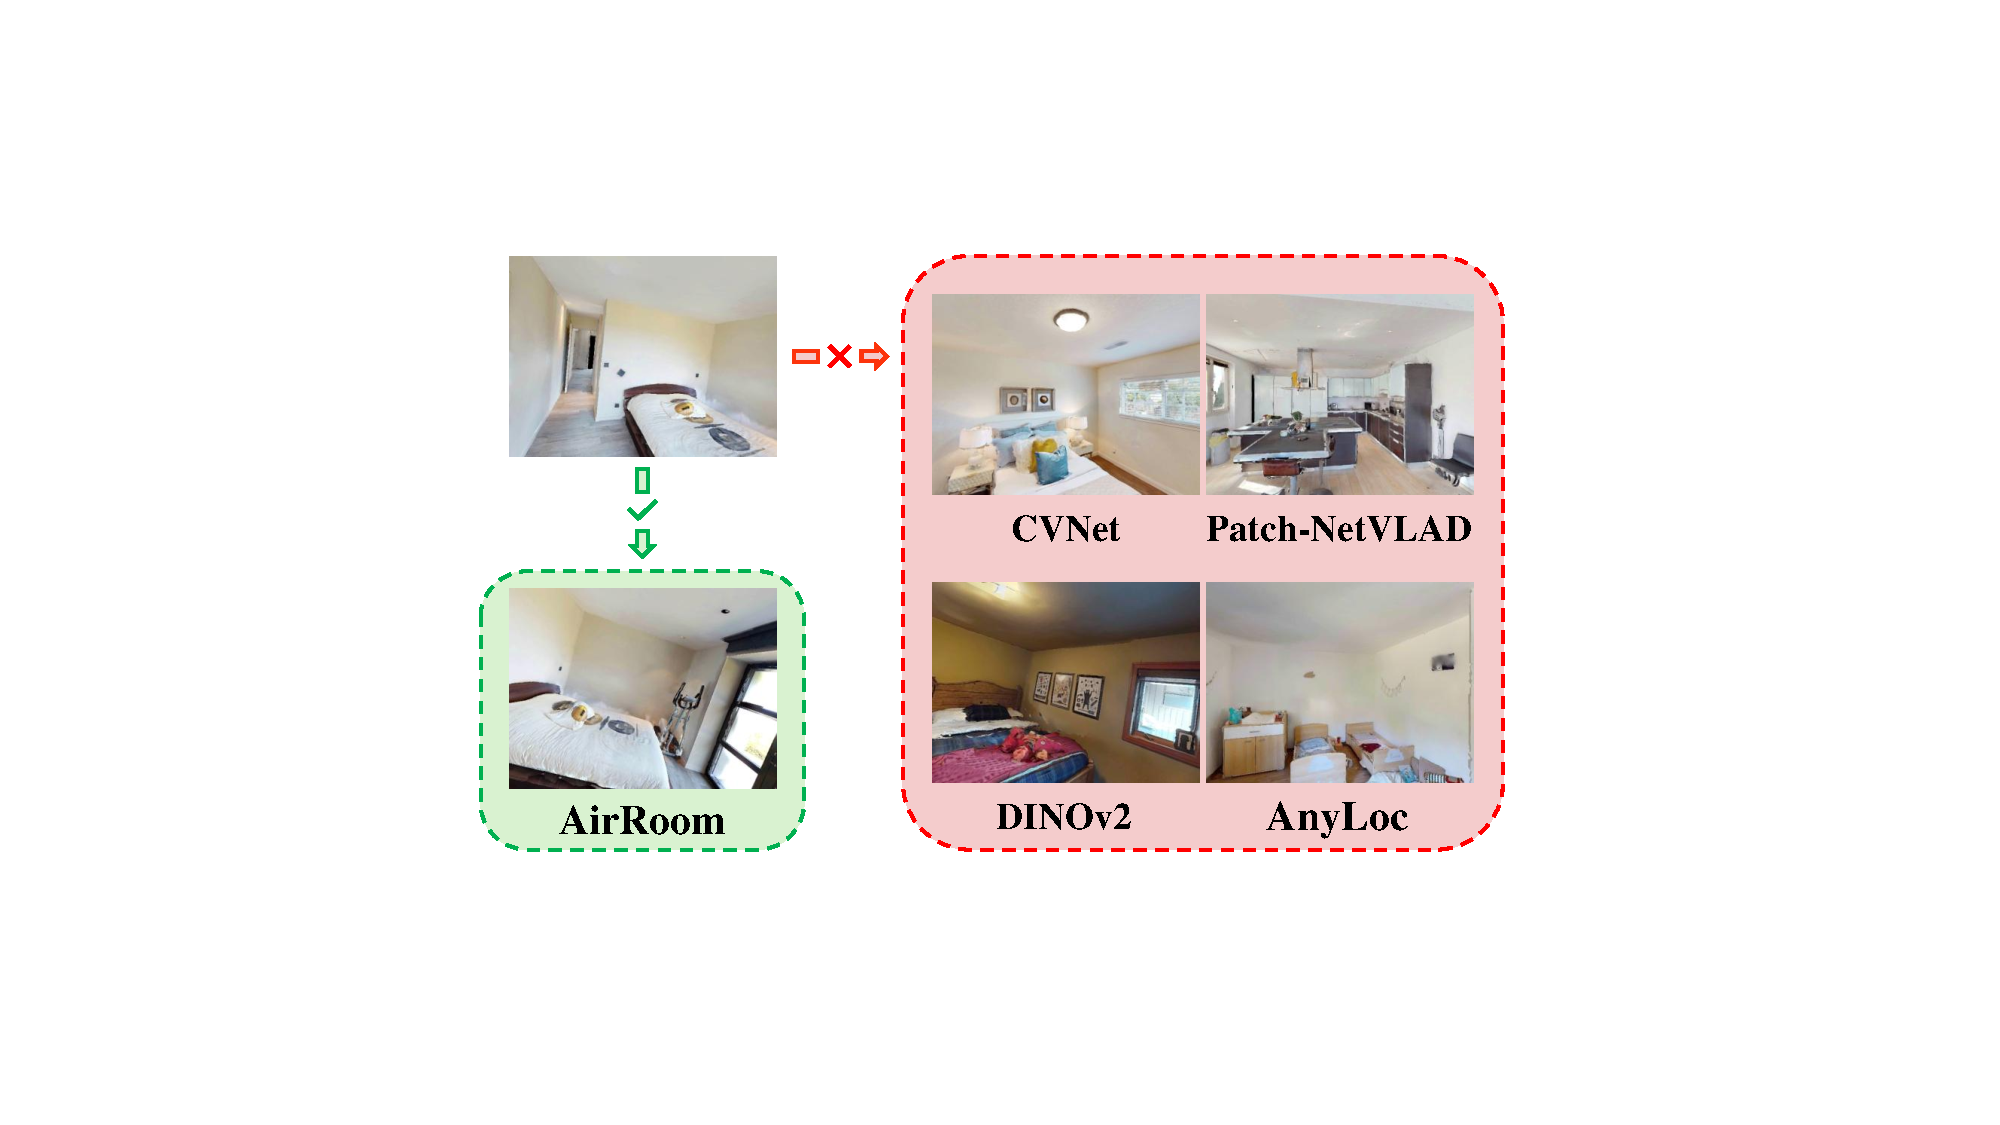
\includegraphics[width=\columnwidth]{failure_font.pdf}
    \vspace{-16pt}
    \caption{给定一个卧室查询,AirRoom 通过利用物体相关性进行房间重识别,准确地检索目标图像。相比之下,CVNet 检索视觉上相似的图像,但没有保持场景的准确性,DINOv2 捕捉语义内容但忽略了颜色细节,Patch-NetVLAD 使用聚合的局部特征形成全局描述符,检索到的图像语义信息不匹配,而 AnyLoc 考虑了语义和颜色属性,但忽略了房间内物体的重要性。}
    \vspace{-5pt}
    \label{fig:failure}
\end{figure}

\tref{tab:overall} 展示了 AirRoom 与基线方法之间的定量比较,结果表明 AirRoom 在几乎所有指标和数据集上均优于所有基线方法。在房间重识别任务中,图像检索方法由于其并非专注于 top-1 精度,通常在分类指标上表现较差,而 VPR 方法则取得了更好的结果。基于全局描述子的 VPR 方法仅捕捉高层语义信息,常常检索到语义相似但缺乏细节的房间;相比之下,使用局部特征聚合的 VPR 方法(如 Patch-NetVLAD)强调低层编码,但可能忽视全局上下文,从而导致检索准确性下降。 \fref{fig:failure} 展示了 CVNet、DINOv2、Patch-NetVLAD 和 AnyLoc 的失败案例,突显了这些方法的局限性。

尽管 AnyLoc 因其在“任何位置、任何时间、任何视角” VPR 中表现稳健而著称,并具有良好性能,但 AirRoom 进一步提升了表现,在可用提升空间内相较 AnyLoc 提高了 20\% 到 40\%。例如,AnyLoc 在 HMReID 上取得了 89.69\% 的准确率,留下了约 10\% 的提升空间;而 AirRoom 凭借 93.80\% 的准确率,在剩余空间内实现了高达 40\% 的提升。这些结果突显了 AirRoom 在房间重识别任务中卓越的精度与优化表现。
\subsection{按组别的性能比较}
\label{sec:section4.5}
\vspace{-3pt}
许多基准方法采用“骨干网络 + 增强机制”的范式,我们的方法也遵循这一范式。在本节中,我们将使用与每个组基准相同的骨干网络,将我们的面向对象增强机制与几种最先进的方法进行性能比较。此设置使我们能够直接评估我们的面向对象增强机制的有效性。

对于ResNet50骨干网络组,我们使用CVNet \cite{lee2022correlationverificationimageretrieval} 作为基准。在NetVLAD骨干网络组中,我们采用Patch-NetVLAD \cite{hausler2021patchnetvladmultiscalefusionlocallyglobal} 作为基准,并在三种降维度下进行测试:4096、512和128。

\tref{tab:grouped}显示,在每个组别中,单一的骨干网络优于那些通过各种机制尝试增强性能的基准方法,这表明这些机制未能有效地捕捉到室内环境中的关键信息。相比之下,我们的面向对象增强机制通过强调室内环境中\mbox{对象}的重要性,显著提升了骨干网络的性能。
\subsection{管道灵活性评估}  
\label{sec:section4.6}  
\vspace{-3pt}  
在本节中,我们通过测试其关键模块的不同配置,系统性地评估了 AirRoom 的灵活性和适应性。结果清楚地表明,AirRoom 并不依赖于任何特定模型,能够有效集成各种不同类型的模型。  

\vspace{-5pt}
\subsubsection{全局特征提取器}
\vspace{-4pt}
我们测试了多种全局特征提取器,包括ViT \cite{dosovitskiy2021imageworth16x16words}、DINO \cite{caron2021emergingpropertiesselfsupervisedvision}、DINOv2 \cite{oquab2024dinov2learningrobustvisual} 和AnyLoc-VLAD-DINOv2 \cite{keetha2023anylocuniversalvisualplace},VLAD簇大小分别为16和8。

如\tref{tab:global feature extractor flexibility}所示,AirRoom在几乎所有情况下,在所有度量标准和数据集上始终能够超过85\%,无论使用的全局特征提取器的能力如何。即使是在DINOv2的唯一例外情况下,AirRoom的表现仍然提高了近15\%。这表明我们的管道的有效性并不依赖于任何特定的全局特征提取器,突显了AirRoom在各种主干配置下的适应性,并强调了其强大的灵活性。

\vspace{-5pt}
\subsubsection{实例分割}
\vspace{-4pt}
我们将传统的实例分割方法(如 Mask R-CNN \cite{he2018maskrcnn})与更近期的 approaches,包括 Semantic-SAM \cite{li2023semanticsamsegmentrecognizegranularity} 进行比较,后者利用先进技术实现更细粒度的分割。

\tref{tab:is flexibility} 显示,无论使用何种实例分割模块,AirRoom 始终比基准方法高出超过 15\%。这证明了我们的管道不依赖于任何特定的实例分割方法,强调了其在此组件中的适应性。

\begin{table}[h]
\vspace{-5pt}
\centering
\resizebox{\columnwidth}{!}{
\begin{tabular}{l|cccc}
\toprule
\multirow{2}{*}{\textbf{Methods}} & \multicolumn{4}{c}{\textbf{HMReID}} \\
 & Accuracy & Precision & Recall & F1 \\
\midrule
DINOv2 & 53.91 & 60.52 & 53.73 & 54.69 \\
\rowcolor{Lavender} AirRoom-MaskRCNN & 69.44 & 72.23 & 69.08 & 69.07 \\
\rowcolor{Lavender} AirRoom-SSAM & \textbf{70.95} & \textbf{73.86} & \textbf{70.66} & \textbf{70.78} \\
\bottomrule
\end{tabular}
}
\vspace{-10pt}
\caption{实例分割的灵活性。}
\vspace{-16pt}
\label{tab:is flexibility}
\end{table}
\subsubsection{目标特征提取器}

我们实验了传统的骨干网络,如 ResNet50 \cite{he2015deepresiduallearningimage},以及更现代的骨干网络,如 DINOv2 \cite{oquab2024dinov2learningrobustvisual},作为目标特征提取器。

如 \tref{tab:ofe flexibility} 所示,AirRoom 在基准模型上实现了显著的性能提升,不同目标特征提取器之间的性能变化很小。这支持了我们管道在适应各种特征提取方法方面的灵活性。

\begin{table}[h]
\vspace{-6pt}
\centering
\resizebox{\columnwidth}{!}{
\begin{tabular}{l|cccc}
\toprule
\multirow{2}{*}{\textbf{Methods}} & \multicolumn{4}{c}{\textbf{HMReID}} \\
 & Accuracy & Precision & Recall & F1 \\
\midrule
DINOv2 & 53.91 & 60.52 & 53.73 & 54.69 \\
\rowcolor{Lavender} AirRoom-ResNet50 & \textbf{70.95} & \textbf{73.86} & \textbf{70.66} & \textbf{70.78} \\
\rowcolor{Lavender} AirRoom-DINOv2 & 68.67 & 71.81 & 68.33 & 68.59 \\
\bottomrule
\end{tabular}
}
\vspace{-10pt}
\caption{目标特征提取器的灵活性。}
\vspace{-20pt}
\label{tab:ofe flexibility}
\end{table}
\subsubsection{面向对象评分}

我们评估了均值 (\(s_{\text{mean}}\)) 和最大值 (\(s_{\max}\)) 两种策略,用于计算补丁得分 (\(s_{\text{patch}}\)) 和对象得分 (\(s_{\text{object}}\)),并评估它们对整体性能的影响。

\tref{tab:os flexibility} 显示,无论使用何种面向对象的评分方法,AirRoom的性能保持稳定。这突显了面向对象信息在房间重新识别中的稳健性,并展示了AirRoom在适应不同评分策略方面的灵活性。

\begin{table}[h]
\vspace{-6pt}
\centering
\resizebox{\columnwidth}{!}{
\begin{tabular}{l|cccc}
\toprule
\multirow{2}{*}{\textbf{Methods}} & \multicolumn{4}{c}{\textbf{HMReID}} \\
 & Accuracy & Precision & Recall & F1 \\
\midrule
DINOv2 & 53.91 & 60.52 & 53.73 & 54.69 \\
\rowcolor{Lavender} AirRoom-Max(patch)-Mean(object) & 70.95 & 73.86 & 70.66 & 70.78 \\
\rowcolor{Lavender} AirRoom-Max(patch)-Max(object) & \textbf{71.02} & \textbf{74.02} & \textbf{70.72} & \textbf{70.85} \\
\rowcolor{Lavender} AirRoom-Mean(patch)-Max(object) & 70.85 & 73.85 & 70.55 & 70.70 \\
\rowcolor{Lavender} AirRoom-Mean(patch)-Mean(object) & 70.90 & 73.78 & 70.62 & 70.73 \\
\bottomrule
\end{tabular}
}
\vspace{-10pt}
\caption{面向对象的评分灵活性。}
\vspace{-20pt}
\label{tab:os flexibility}
\end{table}
\subsection{消融研究}
\label{sec:section4.7}

在本节中,我们从我们的管道中移除某些模块——包括全局得分 \(s_{\text{global}}\)、局部得分 \(s_{\text{patch}}\)、目标得分 \(s_{\text{object}}\)(在目标感知评分中)以及整个细粒度检索(FGR)——以评估每个组件的重要性和有效性。

\begin{table}[t]
\centering
\resizebox{\columnwidth}{!}{
\begin{tabular}{l|cccc}
\toprule
\multirow{2}{*}{\textbf{Methods}} & \multicolumn{4}{c}{\textbf{HMReID}} \\
 & Accuracy & Precision & Recall & F1 \\
\midrule
DINOv2 (AirRoom-w/o all)& 53.91 & 60.52 & 53.73 & 54.69 \\
\rowcolor{Lavender} AirRoom-w/o \(s_{\text{patch}}\) & 66.68 & 70.04 & 66.42 & 66.68 \\
\rowcolor{Lavender} AirRoom-w/o \(s_{\text{object}}\) & 69.77 & 72.84 & 69.48 & 69.64 \\
\rowcolor{Lavender} AirRoom-w/o FGR & 66.11 & 70.85 & 65.80 & 66.41 \\
\rowcolor{Lavender} AirRoom-w/o \(s_{\text{patch}}\) \& \(s_{\text{object}}\) & 62.26 & 66.43 & 62.03 & 62.46 \\
\rowcolor{Lavender} AirRoom-w/o \(s_{\text{patch}}\) \& FGR & 59.39 & 65.25 & 59.14 & 59.97 \\
\rowcolor{Lavender} AirRoom-w/o \(s_{\text{object}}\) \& FGR & 63.44 & 68.68 & 63.14 & 63.84 \\
\rowcolor{Lavender} AirRoom & \textbf{70.95} & \textbf{73.86} & \textbf{70.66} & \textbf{70.78} \\
\bottomrule
\end{tabular}
}
\vspace{-10pt}
\caption{消融研究(不包括全局评分实验)。}
\vspace{-6pt}
\label{tab:ablation w/o global score}
\end{table}

\begin{table}[ht]
\centering
\resizebox{\columnwidth}{!}{
\begin{tabular}{l|cccc}
\toprule
\multirow{2}{*}{\textbf{Methods}} & \multicolumn{4}{c}{\textbf{HMReID}} \\
 & Accuracy & Precision & Recall & F1 \\
\midrule
ViT & 76.47 & 79.37 & 76.04 & 75.91 \\
\rowcolor{Lavender} AirRoom-ViT-w/o \(s_{\text{global}}\) & 84.86 & 86.82 & 84.34 & 84.61 \\
\rowcolor{Lavender} AirRoom-ViT & \textbf{86.58} & \textbf{88.13} & \textbf{86.12} & \textbf{86.23} \\
\cdashline{1-5}
DINOv2 & 53.91 & 60.52 & 53.73 & 54.69 \\
\rowcolor{Lavender} AirRoom-DINOv2-w/o \(s_{\text{global}}\) & \textbf{71.73} & \textbf{74.97} & \textbf{71.44} & \textbf{71.64} \\
\rowcolor{Lavender} AirRoom-DINOv2 & 70.95 & 73.86 & 70.66 & 70.78 \\
\bottomrule
\end{tabular}
}
\vspace{-10pt}
\caption{关于全局得分的消融研究。}
\vspace{-15pt}
\label{tab:ablation on global score}
\end{table}

\tref{tab:ablation w/o global score} 显示,移除任何模块都会导致性能下降。然而,只要至少保留一个模块,我们的管道仍然优于基线。 \tref{tab:ablation on global score} 证明,当全局特征提取器(ViT)表现良好时,全局得分 \(s_{\text{global}}\) 显著提升性能。另一方面,当全局特征提取器(DINOv2)效果较差时,全局得分 \(s_{\text{global}}\) 会产生轻微的负面影响,导致性能略微下降。这个结果与我们在第~\ref{subsec:refinement}节中的假设一致,其中全局得分充当优先级排序的先验,用于排名五个候选者的优先级。总体而言,这些消融研究确认了我们管道中的每个模块都是重要且必要的。
\subsection{局限性}

尽管AirRoom在不同视角变化下的房间重识别任务中达到了最先进的性能,但我们工作的一个局限性是无法验证其对由可移动物体引起的室内物品重排的鲁棒性。尽管我们基于互最近邻的物体感知评分方法在一定程度上对这种重排具有鲁棒性,但我们实验中使用的数据集缺乏这些情况。相比之下,最近在动态场景理解方面的进展 \cite{zhao2024dynamicsceneunderstandingobjectcentric} 专注于在存在移动物体的情况下识别场景,可能比我们的方法提供更强的鲁棒性。未来的工作应考虑构建包含物体重排的数据集,并集成新技术以增强对可移动物体的鲁棒性,从而提高房间重识别的性能。

\vspace{-5pt}
\section{结论}
\vspace{-5pt}
\label{sec:conclusion}

房间重识别是一个具有挑战性但至关重要的研究领域,在增强现实和居家护理机器人等领域的应用不断增长。在本文中,我们提出了AirRoom,这是一种无训练、面向对象的房间重识别方法。AirRoom利用多层次的面向对象特征来捕捉室内房间的空间和上下文信息。为了评估AirRoom,我们专门构建了四个新的数据集用于房间重识别。实验结果证明,AirRoom在视角变化下具有较强的鲁棒性,并且在几乎所有度量和数据集上都优于现有的最先进方法。此外,该管道高度灵活,在不依赖于特定模型配置的情况下仍能保持高性能。总的来说,我们的工作确立了AirRoom作为一种强大且多功能的房间重识别解决方案,具有广泛的现实应用潜力。

\begin{center}
\textbf{致谢}
\end{center}
\begin{sloppypar}
\noindent 本研究得到了 DARPA 资助(奖项编号:HR00112490426)。本文中所表达的任何观点、发现、结论或建议均属于作者本人观点,并不一定代表 DARPA 的立场。
\end{sloppypar}

{
    \small
    \bibliographystyle{ieeenat_fullname}
    \bibliography{main}
}

\clearpage
\setcounter{page}{1}
\maketitlesupplementary

\section{Datasets}
Table \ref{tab:MPReID} presents the composition of MPReID, while Table \ref{tab:HMReID}, Table \ref{tab:GibsonReID}, and Table \ref{tab:ReplicaReID} outline the compositions of HMReID, GibsonReID, and ReplicaReID, respectively. Table \ref{tab:Statistics} reports the number of semantically different rooms in each room ReID dataset.

\begin{table}[ht]
\centering
\vspace{-3pt}
\resizebox{\columnwidth}{!}{
\begin{tabular}{c|c|c|c|c|c}
\toprule
\textbf{Scene} & \textbf{Rooms} & \textbf{Images} & \textbf{Scene} & \textbf{Rooms} & \textbf{Images} \\
\midrule
8WUmhLawc2A & 8 & 1232 & EDJbREhghzL & 7 & 1078 \\
RPmz2sHmrrY & 5 & 770 & S9hNv5qa7GM & 9 & 1423 \\
ULsKaCPVFJR & 5 & 780 & VzqfbhrpDEA & 7 & 1078 \\
WYY7iVyf5p8 & 4 & 616 & X7HyMhZNoso & 7 & 1078 \\
YFuZgdQ5vWj & 7 & 1078 & i5noydFURQK & 7 & 1078 \\
jh4fc5c5qoQ & 5 & 770 & mJXqzFtmKg4 & 9 & 1386 \\
qoiz87JEwZ2 & 8 & 1232 & wc2JMjhGNzB & 11 & 1708 \\
yqstnuAEVhm & 6 & 924 & \textbf{Total} & \textbf{105} & \textbf{16231} \\
\bottomrule
\end{tabular}
}
\vspace{-1em}
\caption{Composition of MPReID.}
\label{tab:MPReID}
\end{table}

\vspace{-1em}

\begin{table}[ht]
\centering
\resizebox{\columnwidth}{!}{
\begin{tabular}{c|c|c|c|c|c}
\toprule
\textbf{Scene} & \textbf{Rooms} & \textbf{Images} & \textbf{Scene} & \textbf{Rooms} & \textbf{Images} \\
\midrule
7dmR22gwQpH & 6 & 924 & ACZZiU6BXLz & 5 & 682 \\
CETmJJqkhcK & 5 & 813 & CFVBbU9Rsyb & 5 & 770 \\
Coer9RdivP7 & 3 & 462 & DZsJKHoqEYg & 5 & 793 \\
EQSguCqe5Rk & 5 & 819 & Fgtk7tL8R9Y & 5 & 822 \\
GLAQ4DNUx5U & 7 & 1156 & GcfUJ79xCZc & 5 & 572 \\
NcK5aACg44h & 5 & 754 & P8L1328HrLi & 5 & 819 \\
VSxVP19Cdyw & 5 & 769 & b3CuYvwpzZv & 5 & 690 \\
ixTj1aTMup2 & 5 & 757 & ochRmQAHtkF & 5 & 641 \\
qWb4MVxqCW7 & 6 & 879 & rrjjmoZhZCo & 5 & 704 \\
w7QyjJ3H9Bp & 5 & 692 & zR6kPe1PsyS & 5 & 803 \\
zepmXAdrpjR & 3 & 460 & \textbf{Total} & \textbf{105} & \textbf{15781} \\
\bottomrule
\end{tabular}
}
\vspace{-1em}
\caption{Composition of HMReID.}
\label{tab:HMReID}
\end{table}

\vspace{-1em}

\begin{table}[ht]
\centering
\resizebox{\columnwidth}{!}{
\begin{tabular}{c|c|c|c|c|c}
\toprule
\textbf{Scene} & \textbf{Rooms} & \textbf{Images} & \textbf{Scene} & \textbf{Rooms} & \textbf{Images} \\
\midrule
Ackermanville & 1 & 154 & Angiola & 1 & 154 \\
Avonia & 2 & 308 & Beach & 3 & 462 \\
Branford & 1 & 154 & Brevort & 1 & 154 \\
Cason & 2 & 262 & Cooperstown & 2 & 308 \\
Corder & 2 & 308 & Creede & 4 & 526 \\
Elmira & 2 & 308 & Eudora & 2 & 308 \\
Fredericksburg & 2 & 308 & Greigsville & 1 & 154 \\
Idanha & 1 & 154 & Laytonsville & 3 & 462 \\
Lynxville & 2 & 308 & Mahtomedi & 2 & 257 \\
Mayesville & 2 & 308 & Northgate & 1 & 154 \\
Ogilvie & 2 & 308 & Ophir & 3 & 462 \\
Pablo & 1 & 154 & Sumas & 2 & 308 \\
- & - & - & \textbf{Total} & \textbf{45} & \textbf{6743} \\
\bottomrule
\end{tabular}
}
\vspace{-1em}
\caption{Composition of GibsonReID.}
\label{tab:GibsonReID}
\end{table}

\vspace{-1em}

\begin{table}[ht]
\centering
\resizebox{\columnwidth}{!}{
\begin{tabular}{c|c|c|c|c|c}
\toprule
\textbf{Scene} & \textbf{Rooms} & \textbf{Images} & \textbf{Scene} & \textbf{Rooms} & \textbf{Images} \\
\midrule
apartment\_0 & 3 & 462 & apartment\_1 & 1 & 154 \\
apartment\_2 & 4 & 616 & frl\_apartment\_0 & 3 & 426 \\
hotel\_0 & 1 & 154 & office\_0 & 1 & 154 \\
office\_2 & 1 & 140 & office\_3 & 1 & 140 \\
office\_4 & 1 & 154 & room\_0 & 1 & 154 \\
room\_1 & 1 & 154 & room\_2 & 1 & 154 \\
- & - & - & \textbf{Total} & \textbf{19} & \textbf{2862} \\
\bottomrule
\end{tabular}
}
\vspace{-1em}
\caption{Composition of ReplicaReID.}
\label{tab:ReplicaReID}
\end{table}

\begin{table}[h]
% \vspace{-10pt}
\centering
\resizebox{\columnwidth}{!}{
\begin{tabular}{c|c|c|c|c|c|c|c|c|c|c|c|c|c|c}
\hline
 & bathroom & kitchen & living & office & bedroom & theater & dining & wardrobe & gym & laundry & garage & storage & nursery & supermarket \\
\hline
MPReID & 13 & 13 & 20 & 3 & 41 & 4 & 4 & 2 & 2 & 2 & 1 & 0 & 0 & 0 \\
\hline
HMReID & 10 & 18 & 29 & 8 & 31 & 0 & 3 & 1 & 0 & 1 & 0 & 2 & 2 & 0 \\
\hline
GibsonReID & 2 & 10 & 11 & 3 & 12 & 0 & 1 & 0 & 3 & 1 & 0 & 1 & 0 & 1 \\
\hline
ReplicaReID & 0 & 2 & 6 & 6 & 3 & 0 & 2 & 0 & 0 & 0 & 0 & 0 & 0 & 0 \\
\hline
\end{tabular}
}
\caption{Statistics of semantically different rooms across four newly constructed room ReID datasets.}
\label{tab:Statistics}
% \vspace{-13pt}
\end{table}

\section{Experimental Details}

\subsection{Overall Performance Comparison}
\label{sec:appendix_overall}

\paragraph{Baseline Configuration} For CVNet, we use ResNet50 as the backbone and set the reduction dimension to 2048. For DINOv2, we utilize the DINOv2-Base checkpoint. For Patch-NetVLAD, we load pre-trained weights optimized on the Pittsburgh dataset, apply WPCA to reduce feature embedding dimensionality to 4096, set RANSAC as the matcher, use patch weights of 0.45, 0.15, and 0.4, configure patch sizes to 2, 5, and 8 with strides of 1 for all. For AnyLoc, we adopt AnyLoc-VLAD-DINOv2 with the DINOv2 ViT-G/14 architecture, set the descriptor layer to 31, use VLAD with 32 clusters, and specify the domain as \mbox{indoor}.

\paragraph{Baseline Adaptation} For CVNet and Patch-NetVLAD, we perform global retrieval by selecting the top-5 candidates, followed by re-ranking. For CVNet, the candidate with the highest CVNet-Rerank image similarity score is chosen as the final result, while for Patch-NetVLAD, the reference with the highest RANSAC score in the Pairwise Local Matching stage is selected. For DINOv2 and AnyLoc, global features are extracted from the query and reference images, and cosine similarity is computed. The reference image with the highest cosine similarity score is selected as the final match.

\paragraph{AirRoom Configuration} For the Global Feature Extractor, we use AnyLoc-VLAD-DINOv2 with the DINOv2 ViT-G/14 architecture, setting the descriptor layer to 31, applying VLAD with 32 clusters, and specifying the domain as indoor. For Instance Segmentation, we employ Semantic-SAM with pre-trained weights from SA-1B and a SwinL backbone. The Object Feature Extractor is implemented using a ResNet50 model pre-trained on the ImageNet dataset. For Fine-Grained Retrieval, we use LightGlue with the maximum number of keypoints set to 2048.

\subsection{Group-Wise Performance Comparison}

\paragraph{Baseline Configuration} For the ResNet50 backbone group, the configurations for ResNet50 and CVNet follow those detailed in \sref{sec:appendix_overall}. For the NetVLAD backbone group, we use NetVLAD with VGG-16 as the feature extractor, configured with 64 clusters and a feature dimensionality of 512. For Patch-NetVLAD, the feature dimensionalities are set to 4096, 512, and 128, respectively, with all other settings consistent with \sref{sec:appendix_overall}.

\paragraph{Baseline Adaptation} For the ResNet50 backbone group, ResNet50 extracts global features from the query and reference images, with cosine similarity used to select the reference image with the highest score as the final match. The adaptation for CVNet is detailed in \sref{sec:appendix_overall}. For the NetVLAD backbone group, NetVLAD aggregates global descriptors from the query and reference local features, and the reference with the highest cosine similarity score is chosen as the final result. The adaptation for Patch-NetVLAD also follows \sref{sec:appendix_overall}.

\paragraph{AirRoom Configuration} For the ResNet50 backbone group, ResNet50 is used as the Global Feature Extractor, with the configuration consistent with \sref{sec:appendix_overall}. For the NetVLAD backbone group, NetVLAD is used as the Global Feature Extractor, following the configuration outlined in the Baseline Configuration paragraph in this section. The configurations for the remaining modules in both groups are also consistent with \sref{sec:appendix_overall}.

\subsection{Pipeline Flexibility Evaluation}

\subsubsection{Global Feature Extractor}

\paragraph{Baseline Configuration} For ViT, we use the Base variant with a patch size of 16 and an input image size of 224×224, loading pre-trained weights from ImageNet. For DINO, we adopt the DINO-pretrained Vision Transformer Small (ViT-S/16) variant. The configuration for DINOv2 follows \sref{sec:appendix_overall}. For AnyLoc, VLAD clusters are set to 16 and 8, with all other configurations consistent with \sref{sec:appendix_overall}.

\paragraph{Baseline Adaptation} All baselines are used to extract features from query and reference images, with cosine similarity computed to identify the reference room with the highest similarity score.

\paragraph{AirRoom Configuration} For comparisons with a backbone baseline, the backbone is used as the Global Feature Extractor. Backbone configurations follow those outlined in the Baseline Configuration paragraph of this section, while the configurations for the remaining modules in AirRoom are consistent with \sref{sec:appendix_overall}.

\subsubsection{Instance Segmentation}

\paragraph{AirRoom Configuration} DINOv2 is used as the Global Feature Extractor. For Mask R-CNN, we use Mask R-CNN with a ResNet50 backbone and FPN, loading pre-trained weights trained on COCO. For Semantic-SAM, we employ Semantic-SAM with pre-trained weights from SA-1B and a SwinL backbone. The configurations for the remaining modules are consistent with \sref{sec:appendix_overall}.

\section{Large-Scale Evaluation}
Since the four room ReID datasets were curated in a consistent format, we evaluate our method on their union, resulting in more examples for each room type and assessing the feasibility of the proposed method when scaling the data. To this end, we construct a large-scale dataset, UnionReID, by combining all four datasets. Table \ref{tab:Union} presents a performance comparison between AirRoom and four baseline methods, demonstrating that AirRoom continues to outperform them under large-scale conditions.

\begin{table}[h]
\centering
\resizebox{\columnwidth}{!}{
\begin{tabular}{l|cccc}
\toprule
\multirow{2}{*}{\textbf{Methods}} & \multicolumn{4}{c}{\textbf{UnionReID}} \\
 & Accuracy & Precision & Recall & F1 \\
\midrule
CVNet & 14.10 & 27.53 & 14.10 & 16.19 \\
DINOv2 & 53.01 & 59.44 & 53.02 & 53.50 \\
Patch-NetVLAD & 61.15 & 67.53 & 61.04 & 62.31 \\
AnyLoc & 88.28 & 89.62 & 88.22 & 88.32 \\
\rowcolor{Lavender} AirRoom & \textbf{91.87} & \textbf{92.55} & \textbf{91.76} & \textbf{91.76} \\
\bottomrule
\end{tabular}
}
\caption{Comparison with baseline models on UnionReID to evaluate AirRoom's performance under data scaling.}
\label{tab:Union}
\end{table}

\section{Evaluation on Indoor Localization Datasets}
Strictly speaking, room ReID is a novel task with no previously established datasets and is fundamentally distinct from indoor localization. To address this gap, we introduced four new datasets. However, after reviewing existing indoor localization datasets, we identified two that are marginally usable: InLoc  \cite{taira2018inlocindoorvisuallocalization} and Structured3D \cite{Structured3D}. InLoc \cite{taira2018inlocindoorvisuallocalization} employs area-based rather than room-based splits, with some images capturing only corridors and corners. Structured3D \cite{Structured3D} contains tens of thousands of room instances, but each room has fewer than six viewpoints. These limitations reduce the suitability of these two datasets, though they remain partially usable. Nonetheless, evaluating our method on them can further reinforce its validation.

Table \ref{tab:Indoor} presents the comparison results on the two indoor localization datasets, where AirRoom continues to outperform other methods. Additionally, as InLoc represents a more realistic real-world setting, the results further demonstrate AirRoom's robustness in practical environments.

\begin{table}[h]
\vspace{-7pt}
\centering
\resizebox{\columnwidth}{!}{
\begin{tabular}{l|cccc|cccc}
\toprule
\multirow{2}{*}{\textbf{Methods}} & \multicolumn{4}{c|}{\textbf{InLoc}} & \multicolumn{4}{c}{\textbf{Structured3D}} \\
 & Acc & Prec & Rec & F1 & Acc & Prec & Rec & F1 \\
\midrule
CVNet & 8.41 & 12.49 & 8.41 & 8.99 & 12.60 & 21.39 & 12.60 & 14.22 \\
DINOv2 & 11.13 & 19.93 & 11.13 & 11.85 & 53.00 & 63.60 & 53.00 & 54.04 \\
Patch-NetVLAD & 12.78 & 19.59 & 12.78 & 13.73 & 56.30 & 67.67 & 56.30 & 57.71 \\
AnyLoc & 15.78 & 26.11 & 15.78 & 17.04 & 73.40 & 79.75 & 73.40 & 73.90 \\
\rowcolor{Lavender} AirRoom & \textbf{16.80} & \textbf{26.36} & \textbf{16.80} & \textbf{18.05} & \textbf{76.20} & \textbf{82.88} & \textbf{76.20} & \textbf{76.70} \\
\bottomrule
\end{tabular}
}
\caption{Comparison with baseline models on existing datasets to further validate our method.}
\label{tab:Indoor}
\end{table}

\section{Runtime Analysis}

In this section, we evaluate the runtime of each module and compare the total runtime of our pipeline with several state-of-the-art methods to assess the efficiency of our approach.

\begin{table}[ht]
\centering
\resizebox{\columnwidth}{!}{%
\begin{tabular}{l|cccccc}
\toprule
\multirow{2}{*}{\textbf{Modules}} & \multicolumn{6}{c}{\textbf{Runtime (ms)}} \\
 & t=0 & t=0.1 & t=0.2 & t=0.3 & t=0.4 & t=0.5 \\
\midrule
Global Feature Extractor & 48.8 & 44.1 & 43.2 & 44.0 & 43.0 & 43.8 \\
Global Retrieval & 0.1 & 0.1 & 0.1 & 0.1 & 0.1 & 0.1 \\
Instance Segmentation & 38.7 & 38.1 & 38.2 & 38.1 & 38.0 & 38.0 \\
Receptive Field Expander & 6.9 & 2.9 & 1.7 & 1.3 & 0.9 & 0.7 \\
Object Feature Extractor & 113.7 & 71.3 & 47.0 & 33.3 & 29.0 & 22.8 \\
Object-Aware Scoring & 2.9 & 2.2 & 1.7 & 1.5 & 1.4 & 1.2 \\
Fine-Grained Retrieval & 87.4 & 86.3 & 86.1 & 86.1 & 85.8 & 86.2 \\
\midrule
\textbf{Total} & \textbf{299.9} & \textbf{246.5} & \textbf{219.4} & \textbf{205.7} & \textbf{199.5} & \textbf{194.2} \\
\bottomrule
\end{tabular}%
}
\caption{Mask R-CNN \& ResNet Runtime.}
\label{tab:module_runtime_mr}
\end{table}

\begin{table}[ht]
\centering
\resizebox{\columnwidth}{!}{%
\begin{tabular}{l|cccccc}
\toprule
\multirow{2}{*}{\textbf{Modules}} & \multicolumn{6}{c}{\textbf{Runtime (ms)}} \\
 & t=0 & t=0.1 & t=0.2 & t=0.3 & t=0.4 & t=0.5 \\
\midrule
Global Feature Extractor & 65.0 & 58.6 & 52.7 & 50.2 & 48.6 & 47.9 \\
Global Retrieval & 0.1 & 0.1 & 0.1 & 0.1 & 0.1 & 0.1 \\
Instance Segmentation & 38.4 & 38.8 & 38.6 & 38.7 & 38.6 & 38.5 \\
Receptive Field Expander & 7.9 & 3.2 & 1.8 & 1.3 & 1.0 & 0.7 \\
Object Feature Extractor & 146.9 & 86.9 & 55.6 & 40.9 & 32.3 & 26.3 \\
Object-Aware Scoring & 2.9 & 2.2 & 1.7 & 1.5 & 1.4 & 1.2 \\
Fine-Grained Retrieval & 87.0 & 87.4 & 87.0 & 87.1 & 87.5 & 87.3 \\
\midrule
\textbf{Total} & \textbf{349.5} & \textbf{278.6} & \textbf{238.8} & \textbf{221.1} & \textbf{210.9} & \textbf{203.4} \\
\bottomrule
\end{tabular}%
}
\caption{Mask R-CNN \& DINOv2 Runtime.}
\label{tab:module_runtime_md}
\end{table}

\begin{table}[ht]
\centering
\resizebox{\columnwidth}{!}{%
\begin{tabular}{l|cccccc}
\toprule
\multirow{2}{*}{\textbf{Methods}} & \multicolumn{6}{c}{\textbf{Accuracy (\%)}} \\
 & t=0 & t=0.1 & t=0.2 & t=0.3 & t=0.4 & t=0.5 \\
\midrule
AirRoom-MaskRCNN-ResNet & 92.70 & 92.68 & 92.58 & 92.59 & 92.22 & 92.15 \\
AirRoom-MaskRCNN-DINOv2 & 87.67 & 87.62 & 87.10 & 87.20 & 87.24 & 87.09 \\
\bottomrule
\end{tabular}%
}
\caption{Mask R-CNN \& ResNet / DINOv2 Accuracy.}
\label{tab:module_accuracy}
\end{table}

\begin{figure}[ht]
    \centering
    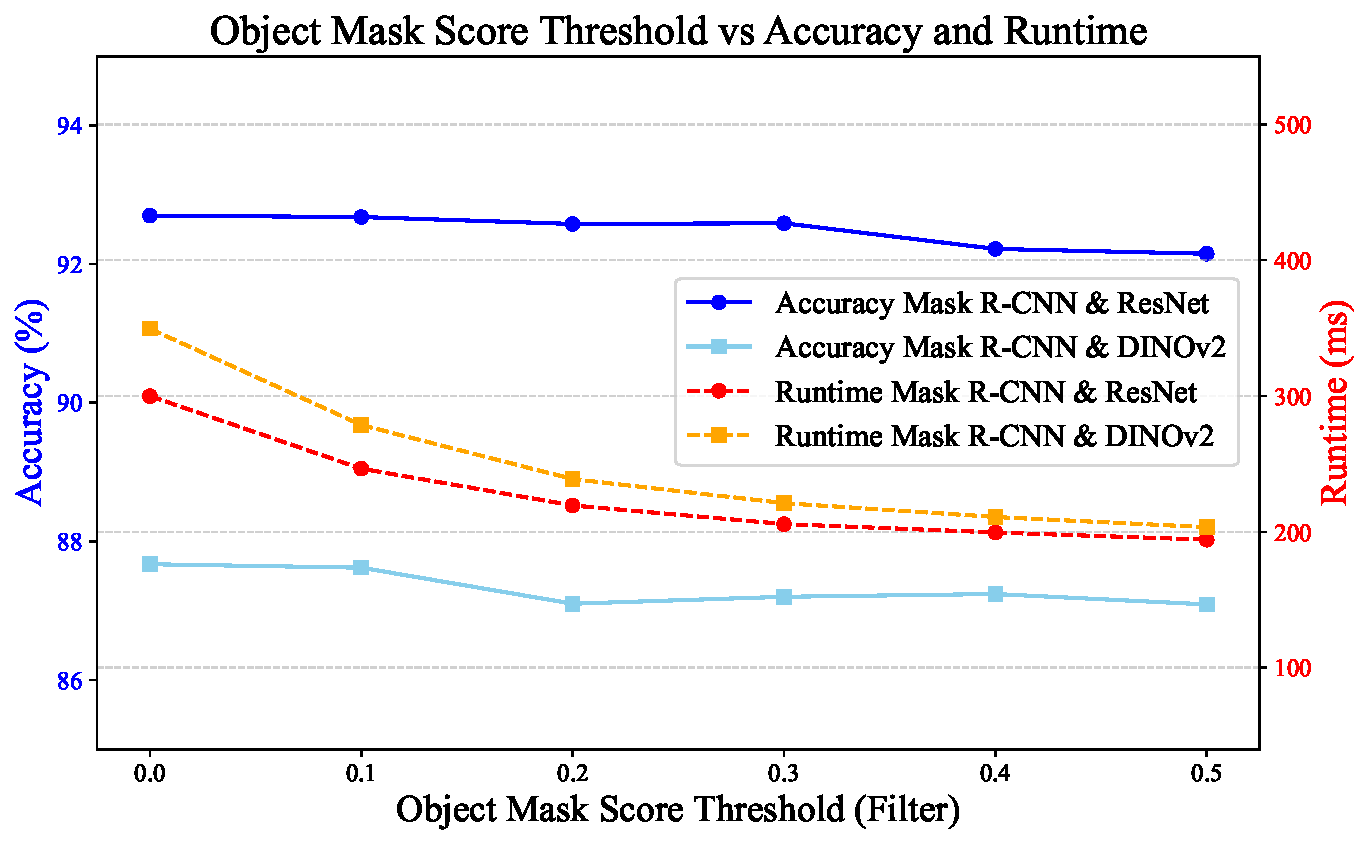
\includegraphics[width=\columnwidth]{runtime.pdf}
    \caption{As the object mask score threshold increases, AirRoom's performance experiences a slight decline; however, the efficiency improves significantly.}
    \label{fig:runtime}
\end{figure}

\begin{table}[ht]
\centering
\begin{tabular}{l|cc}
\toprule
\multirow{2}{*}{\textbf{Modules}} & \multicolumn{2}{c}{\textbf{Runtime (ms)}} \\
 & ResNet & DINOv2 \\
\midrule
Global Feature Extractor & 42.5 & 56.2 \\
Global Retrieval & 0.1 & 0.1 \\
Instance Segmentation & 352.6 & 343.2 \\
Receptive Field Expander & 0.7 & 0.6 \\
Object Feature Extractor & 51.1 & 66.6 \\
Object-Aware Scoring & 2.2 & 2.1 \\
Fine-Grained Retrieval & 87.8 & 87.4 \\
\midrule
\textbf{Total} & \textbf{538.5} & \textbf{557.6} \\
\bottomrule
\end{tabular}%
\caption{Semantic-SAM \& ResNet / DINOv2 Runtime.}
\label{tab:module_runtime_ssam}
\end{table}

\begin{table}[ht]
\centering
\begin{tabular}{l|c|c}
\toprule
\textbf{Methods} & \textbf{Runtime (ms)} & \textbf{Accuracy (\%)}\\
\midrule
CVNet & 111.3 & 11.71 \\
DINOv2 & \textbf{16.7} & 53.91 \\
Patch-NetVLAD & 100.5 & 64.86 \\
AnyLoc & 45.5 & 89.69 \\
\rowcolor{Lavender} AirRoom & 194.2 & \textbf{92.15} \\
\bottomrule
\end{tabular}
\caption{Runtime Comparison with State-of-the-Art Methods.}
\label{tab:runtime_comparison}
\end{table}

When Mask R-CNN is used for instance segmentation, \tref{tab:module_runtime_mr} demonstrates that increasing the object mask score threshold significantly reduces the runtime of the Object Feature Extractor when ResNet is employed. This is attributed to the reduced number of objects and patches requiring processing. A similar trend is observed with DINOv2 as the Object Feature Extractor, as shown in \tref{tab:module_runtime_md}. Additionally, \tref{tab:module_accuracy} indicates that AirRoom's performance remains largely unaffected by the rise in the object mask score threshold, regardless of the chosen Object Feature Extractor. This observation is further illustrated in \fref{fig:runtime}. However, when Semantic-SAM is used for instance segmentation, AirRoom faces efficiency challenges due to Semantic-SAM's significantly slower performance, as detailed in \tref{tab:module_runtime_ssam}.

\tref{tab:runtime_comparison} compares runtime across methods. AirRoom requires 80ms more than CVNet but achieves over 80\% performance improvement. Compared to Patch-NetVLAD, AirRoom's runtime is approximately double, with a performance gain exceeding 30\%. While DINOv2 completes tasks in 10–20ms, AirRoom adds 170ms and improves performance by over 40\%. Relative to AnyLoc, AirRoom increases runtime by just over 150ms but captures an additional 20\% of the remaining performance potential. These results demonstrate that AirRoom delivers significant performance gains even within limited improvement margins, underscoring its effectiveness despite incremental runtime.

Currently, AirRoom allocates approximately 90ms to Fine-Grained Retrieval, utilizing LightGlue for feature matching. Exploring more lightweight and faster alternatives could further enhance efficiency. In real-world applications such as Real-Time Navigation, room reidentification times between 50–200ms are generally acceptable, with accuracy as the primary concern. While AirRoom is slightly slower than some baselines, it achieves substantial accuracy improvements, effectively balancing runtime and performance. This makes AirRoom well-suited for practical scenarios, meeting real-world runtime requirements while maintaining high reliability and precision.

\end{document}
